%File: anonymous-submission-latex-2025.tex
\documentclass[letterpaper]{article} % DO NOT CHANGE THIS
\usepackage[submission]{aaai25}  % DO NOT CHANGE THIS
\usepackage{times}  % DO NOT CHANGE THIS
\usepackage{helvet}  % DO NOT CHANGE THIS
\usepackage{courier}  % DO NOT CHANGE THIS
\usepackage[hyphens]{url}  % DO NOT CHANGE THIS
\usepackage{graphicx} % DO NOT CHANGE THIS
\urlstyle{rm} % DO NOT CHANGE THIS
\def\UrlFont{\rm}  % DO NOT CHANGE THIS
\usepackage{natbib}  % DO NOT CHANGE THIS AND DO NOT ADD ANY OPTIONS TO IT
\usepackage{caption} % DO NOT CHANGE THIS AND DO NOT ADD ANY OPTIONS TO IT
\frenchspacing  % DO NOT CHANGE THIS
\setlength{\pdfpagewidth}{8.5in} % DO NOT CHANGE THIS
\setlength{\pdfpageheight}{11in} % DO NOT CHANGE THIS
%
% These are recommended to typeset algorithms but not required. See the subsubsection on algorithms. Remove them if you don't have algorithms in your paper.
\usepackage{algorithm}
%\usepackage{algorithmic}
\usepackage{lipsum}
\usepackage{amsmath}
\usepackage{amssymb}
\usepackage{amsthm}
\usepackage{listings}
\usepackage{algorithm}
\usepackage{algpseudocode}
\usepackage{booktabs}
\usepackage{enumitem}
%
% These are are recommended to typeset listings but not required. See the subsubsection on listing. Remove this block if you don't have listings in your paper.
\usepackage{newfloat}
\usepackage{listings}
\DeclareCaptionStyle{ruled}{labelfont=normalfont,labelsep=colon,strut=off} % DO NOT CHANGE THIS
\lstset{%
	basicstyle={\footnotesize\ttfamily},% footnotesize acceptable for monospace
	numbers=left,numberstyle=\footnotesize,xleftmargin=2em,% show line numbers, remove this entire line if you don't want the numbers.
	aboveskip=0pt,belowskip=0pt,%
	showstringspaces=false,tabsize=2,breaklines=true}
\floatstyle{ruled}
\newfloat{listing}{tb}{lst}{}
\floatname{listing}{Listing}
%
% Keep the \pdfinfo as shown here. There's no need
% for you to add the /Title and /Author tags.
\pdfinfo{
/TemplateVersion (2025.1)
}

% DISALLOWED PACKAGES
% \usepackage{authblk} -- This package is specifically forbidden
% \usepackage{balance} -- This package is specifically forbidden
% \usepackage{color (if used in text)
% \usepackage{CJK} -- This package is specifically forbidden
% \usepackage{float} -- This package is specifically forbidden
% \usepackage{flushend} -- This package is specifically forbidden
% \usepackage{fontenc} -- This package is specifically forbidden
% \usepackage{fullpage} -- This package is specifically forbidden
% \usepackage{geometry} -- This package is specifically forbidden
% \usepackage{grffile} -- This package is specifically forbidden
% \usepackage{hyperref} -- This package is specifically forbidden
% \usepackage{navigator} -- This package is specifically forbidden
% (or any other package that embeds links such as navigator or hyperref)
% \indentfirst} -- This package is specifically forbidden
% \layout} -- This package is specifically forbidden
% \multicol} -- This package is specifically forbidden
% \nameref} -- This package is specifically forbidden
% \usepackage{savetrees} -- This package is specifically forbidden
% \usepackage{setspace} -- This package is specifically forbidden
% \usepackage{stfloats} -- This package is specifically forbidden
% \usepackage{tabu} -- This package is specifically forbidden
% \usepackage{titlesec} -- This package is specifically forbidden
% \usepackage{tocbibind} -- This package is specifically forbidden
% \usepackage{ulem} -- This package is specifically forbidden
% \usepackage{wrapfig} -- This package is specifically forbidden
% DISALLOWED COMMANDS
% \nocopyright -- Your paper will not be published if you use this command
% \addtolength -- This command may not be used
% \balance -- This command may not be used
% \baselinestretch -- Your paper will not be published if you use this command
% \clearpage -- No page breaks of any kind may be used for the final version of your paper
% \columnsep -- This command may not be used
% \newpage -- No page breaks of any kind may be used for the final version of your paper
% \pagebreak -- No page breaks of any kind may be used for the final version of your paperr
% \pagestyle -- This command may not be used
% \tiny -- This is not an acceptable font size.
% \vspace{- -- No negative value may be used in proximity of a caption, figure, table, section, subsection, subsubsection, or reference
% \vskip{- -- No negative value may be used to alter spacing above or below a caption, figure, table, section, subsection, subsubsection, or reference

\setcounter{secnumdepth}{0} %May be changed to 1 or 2 if section numbers are desired.

% The file aaai25.sty is the style file for AAAI Press
% proceedings, working notes, and technical reports.
%

% Title

% Your title must be in mixed case, not sentence case.
% That means all verbs (including short verbs like be, is, using,and go),
% nouns, adverbs, adjectives should be capitalized, including both words in hyphenated terms, while
% articles, conjunctions, and prepositions are lower case unless they
% directly follow a colon or long dash
\title{When to Accept Automated Predictions and \\ When to Defer to Human Judgment?}
\author{
    %Authors
    % All authors must be in the same font size and format.
    Written by AAAI Press Staff\textsuperscript{\rm 1}\thanks{With help from the AAAI Publications Committee.}\\
    AAAI Style Contributions by Pater Patel Schneider,
    Sunil Issar,\\
    J. Scott Penberthy,
    George Ferguson,
    Hans Guesgen,
    Francisco Cruz\equalcontrib,
    Marc Pujol-Gonzalez\equalcontrib
}
\affiliations{
    %Afiliations
    \textsuperscript{\rm 1}Association for the Advancement of Artificial Intelligence\\
    % If you have multiple authors and multiple affiliations
    % use superscripts in text and roman font to identify them.
    % For example,

    % Sunil Issar\textsuperscript{\rm 2},
    % J. Scott Penberthy\textsuperscript{\rm 3},
    % George Ferguson\textsuperscript{\rm 4},
    % Hans Guesgen\textsuperscript{\rm 5}
    % Note that the comma should be placed after the superscript

    1101 Pennsylvania Ave, NW Suite 300\\
    Washington, DC 20004 USA\\
    % email address must be in roman text type, not monospace or sans serif
    proceedings-questions@aaai.org
%
% See more examples next
}

%Example, Single Author, ->> remove \iffalse,\fi and place them surrounding AAAI title to use it
\iffalse
\title{My Publication Title --- Single Author}
\author {
    Author Name
}
\affiliations{
    Affiliation\\
    Affiliation Line 2\\
    name@example.com
}
\fi

\iffalse
%Example, Multiple Authors, ->> remove \iffalse,\fi and place them surrounding AAAI title to use it
\title{My Publication Title --- Multiple Authors}
\author {
    % Authors
    First Author Name\textsuperscript{\rm 1},
    Second Author Name\textsuperscript{\rm 2},
    Third Author Name\textsuperscript{\rm 1}
}
\affiliations {
    % Affiliations
    \textsuperscript{\rm 1}Affiliation 1\\
    \textsuperscript{\rm 2}Affiliation 2\\
    firstAuthor@affiliation1.com, secondAuthor@affilation2.com, thirdAuthor@affiliation1.com
}
\fi


% REMOVE THIS: bibentry
% This is only needed to show inline citations in the guidelines document. You should not need it and can safely delete it.
\usepackage{bibentry}
% END REMOVE bibentry

\begin{document}

\maketitle

% Uncomment the following to link to your code, datasets, an extended version or similar.
%
% \begin{links}
%     \link{Code}{https://aaai.org/example/code}
%     \link{Datasets}{https://aaai.org/example/datasets}
%     \link{Extended version}{https://aaai.org/example/extended-version}
% \end{links}

%%%%%%%%%%%%
% SECTIONS %
%%%%%%%%%%%%

%%%%%%%%%%%%
% ABSTRACT %
%%%%%%%%%%%%

\begin{abstract}
Ensuring the reliability and safety of automated decision-making is crucial.
This paper proposes a new approach for measuring the reliability of predictions in machine learning models.
We analyze how the softmax outputs of a trained neural network change using clustering to measure Euclidean distances between softmax  outputs and class centroids.
We propose this distance as a metric to evaluate the confidence of predictions.
We assign each prediction to a cluster with centroid representing the mean softmax output for all correct predictions of a given class.
We then define a safety threshold for a class as the smallest distance from an incorrect prediction to the given class centroid.
We evaluate the approach on the MNIST and CIFAR-10 datasets using a Convolutional Neural Network and a Vision Transformer, respectively.
The results show that our approach is consistent across these data sets and network models, and indicate that the proposed metric can offer an efficient way of determining when automated predictions are acceptable and when they should be deferred to human operators.    
\end{abstract} 
%%%%%%%%%%%%%%%%
% INTRODUCTION %
%%%%%%%%%%%%%%%%

\section{Introduction}

Ensuring the reliability and safety of automated decision-making systems is important, particularly in high-impact areas where there exists potential for significant harm from errors \cite{amodei2016concrete}. Machine learning (ML) models, while powerful, are susceptible to making erroneous predictions when faced with data that differs from the distribution that they were trained on \cite{hendrycks2021many}. This phenomenon, known as distribution shift, poses a significant challenge in deploying ML in real-world scenarios \cite{quinonero2009dataset}.

Distribution shift is a pervasive issue in ML, occurring when the distribution of the data used to train a model differs from the distribution of the data that the model encounters during deployment \cite{quinonero2009dataset}. This discrepancy can lead to a significant degradation in model performance, as it may struggle to generalize to the new, unseen data \cite{hendrycks2019benchmarking}. 

Distribution shifts can manifest in various forms, such as covariate shift, concept drift, and domain shift \cite{moreno2012unifying}. Covariate shift arises when the input data distribution changes while the conditional distribution of the output given the input remains the same \cite{shimodaira2000improving}. Concept drift occurs when the relationship between the input and output variables changes over time \cite{gama2014survey}. Domain shift refers to the situation where the model is trained on data from one domain but applied to data from a different domain \cite{patel2015visual}.

To quantify and address distribution shift, researchers have developed various metrics and techniques. One common approach is to use statistical divergence measures, such as Kullback-Leibler (KL) divergence \cite{kullback1951information} or Maximum Mean Discrepancy (MMD) \cite{gretton2012kernel}, to assess differences in training and test data distributions. These metrics provide a quantitative understanding of the extent of the distribution shift.

Another approach is to employ domain adaptation techniques, which aim to align the feature distributions of the source and target domains \cite{wang2018deep}. This can be achieved through methods such as importance weighting \cite{sugiyama2007covariate}, feature transformation \cite{pan2009survey}, or adversarial learning \cite{ganin2016domain}. These techniques seek to mitigate the impact of distribution shift by making the model more robust to changes in the data distribution.

Recent work has also focused on developing algorithms that can detect and adapt to distribution shift in real-time \cite{lu2018learning}. These methods often rely on monitoring the model's performance on a stream of data and adjusting the model's parameters or architecture when a significant drop in performance is detected \cite{baena2006early}. Such adaptive approaches are particularly relevant in dynamic environments where the data distribution is likely to change over time.

Therefore, distribution shift is a significant challenge  that can lead to poor model performance if not addressed properly. %Researchers have proposed various metrics and techniques to quantify and mitigate the impact of distribution shift, ranging from statistical divergence measures to domain adaptation and adaptive algorithms. 
As ML models are increasingly deployed in real-world applications, developing robust methods to handle distribution shift remains an important area of research.

%Leaving aside domain adaptation, we can see that there are approaches based on measuring the shift and approaches based on measuring the drop in accuracy. In this paper we seek to relate/combine the two? Use both to find a threshold... we need to say what the benefit is here.

%Maybe we can say this: neural network predictions, different from other (Bayesian) ML approaches do not offer a measure of confidence in the predictions. Confidence in the prediction is key to deal with the problem of distribution shift. It has been argued recently that \textit{knowing when the system does not know} should be a main metric for ML \cite{DBLP:conf/uai/VentolaB0MK23}. The relationships established in this paper between metric-based and model performance approaches to  distribution shift seek to offer such a connection between accuracy and confidence values. A trained network that has minimized entropy in a softmax layer offers a window into the link between accuracy and confidence values in that a lower entropy should indicate a higher class discrimination (a \textit{pointy} softmax distribution) and a higher entropy should correspond to a softmax distribution that is closer to the uniform distribution. By investigating how the softmax distribution changes with different forms of distribution shift (different types of noise systematically added to the data) we are able to identify trends in the drop of accuracy over time in comparison with the usual distribution shift metrics such as KL divergence. As a result of the above analysis of accuracy and confidence, we are able to define a confidence threshold as the distance from class centroids (explained next) to the first false positive example in the test set. Beyond this threshold, predictions should be deferred to human judgement. In practice, the threshold may vary from an application to another depending on the criticality of the task and the risk of making a wrong decision. 

In this paper, we propose a novel approach for quantifying the reliability of predictions made by neural networks under distribution shift. Our method leverages clustering techniques to measure the distances between the outputs of a trained neural network and class centroids in the softmax distance space. By analyzing these distances, we develop a metric that provides insight into the confidence that one may attribute to the model's predictions. We adopt the most conservative threshold value at which model predictions are expected to be 100\% accurate. The proposed metric offers a computationally efficient, practical way to determine when to accept an automated prediction and when human intervention may be necessary.
%, though in some time-critical scenarios, asking a human for information may not be an option \cite{amodei2016concrete}.

Furthermore, we explore the relationship between the distance to class centroids and the model's predictive accuracy. Our findings confirm as expected that classes predicted more accurately by the model tend to have lower softmax distances to their respective centroids. This observation highlights the potential for using the changes observed in the softmax distribution as a proxy for our confidence in the model's predictions. The objective is to establish a closer link than thus far identified by the literature between the distance-based metrics proposed for distribution shift and the approaches that measure the drop in model accuracy. It is expected to offer a better understanding of the connection between model performance and reliability, that is, accuracy and how confident we are in the predictions of neural networks. 

%NEED TO SUMMARISE THE RESULTS HERE: SAY THAT CNN AND VIT WERE USED, THE APPROACH IS EFFICIENT / LIGHTWEIGHT / SCALES WELL AND THE RESULTS ARE CONSISTENT FOR CNN AND VIT... 

%We can't claim this yet:
%The implications of our work extend beyond the realm of image classification. We are currently applying these concepts to enhance the safety of autonomous systems, specifically in the context of self-driving cars using the CARLA simulator. By identifying scenarios where human judgment is preferable to the autonomous system's assessment, our methodology aims to improve the overall safety and reliability of decision-making in complex, real-world environments.

The main contributions of this paper are:
\begin{itemize}
\item A new lightweight approach for quantifying the reliability of neural networks under distribution shift using distance metrics and clustering to take full advantage of the learned softmax distributions.
\item A combined analysis of the metric-based and accuracy-based methods to tackle distribution shift, with experimental results showing consistency of the proposed approach across CNN and ViT architectures.
\end{itemize}

% You can make this disclaimer shorter maybe as a footnote, because the paper is more about the accuracy versus confidence argument than real systems. 

While identifying and mitigating safety risks within the classification model itself is crucial, it does not guarantee the overall safety, robustness, reliability, trustworthiness, and confident performance of the entire system in which the model is deployed. In critical applications, the classification model is often just one component of a larger, complex system.

% \subsection{Disclaimer}

% While identifying and mitigating safety risks within the classification model itself is crucial, it does not guarantee the overall safety, robustness, reliability, trustworthiness, and confident performance of the entire system in which the model is deployed.

% In critical applications, the classification model is often just one component of a larger, complex system. The safe and reliable operation of such a system depends on the proper functioning and interaction of all its components, including data acquisition, preprocessing, decision-making, and actuation. Even if the classification model is designed to mitigate safety risks, failures or vulnerabilities in other components can still compromise the overall safety and reliability of the system.

% Furthermore, the deployment environment and context in which the classification system operates can introduce additional challenges and risks that may not be fully captured or addressed during the model development phase. Factors such as data distribution shifts, adversarial attacks, or unexpected edge cases can impact the model's performance and lead to potential safety issues.

% Therefore, it is important to recognize that developing a safe and reliable classification model is necessary but not sufficient for ensuring the overall safety and reliability of the deployed system. A holistic approach that considers the entire system architecture, interfaces, and deployment context is essential. This includes rigorous testing, validation, and monitoring of the entire system, as well as establishing robust failsafe mechanisms and human oversight to handle unexpected situations and maintain safe operation.

% In summary, while identifying and mitigating safety risks within the classification model is important, it is crucial to acknowledge that it does not guarantee the safe and reliable performance of the entire deployed system. A comprehensive approach considering all components, their interactions, and the deployment context is necessary to ensure the safe, robust, reliable, trustworthy, and confident operation of critical applications.


 
%%%%%%%%%%%
% CONTEXT %
%%%%%%%%%%%

\section{Background}

%%%%%%%%%%%%%%%%%%%%
% SOFTMAX DISTANCE %
%%%%%%%%%%%%%%%%%%%%

% SOFTMAX DISTANCE USED AS ANOMALY DETECTION

% The concept of using the entire set of softmax prediction probabilities, rather than solely relying on the maximum output, has been extensively studied in the context of enhancing the safety, robustness, and trustworthiness of machine learning models. By considering the complete distribution of class predictions provided by the softmax output, more reliable and informative prediction pipelines may be developed, that go beyond point estimates. This approach enables the exploration of uncertainty quantification, anomaly detection, and other techniques that contribute to building safer, more robust, and trustworthy autonomous systems.
% \citet{hendrycks2018baseline} proposed a softmax prediction probability baseline for error and out-of-distribution detection across various architectures and datasets. \citet{klaus2022anomaly} uses the mean parameters of softmax function prior distribution as the cluster centroids, and unlike our approach do not use k-means to generate centroids and cluster assignments.

\textbf{Softmax prediction probabilities}: The concept of using the entire set of softmax prediction probabilities, rather than solely relying on the maximum output, has been extensively studied in the context of enhancing the safety, robustness, and trustworthiness of machine learning models. By considering the complete distribution of class predictions provided by the softmax output, more reliable and informative prediction pipelines may be developed, that go beyond point estimates \cite{gal2016dropout}. This approach enables the exploration of uncertainty quantification, anomaly detection, and other techniques that contribute to building safer, more robust, and trustworthy autonomous systems.

Uncertainty quantification is a crucial aspect of reliable machine learning systems, as it allows for the estimation of confidence in the model's predictions \cite{kendall2017uncertainties}. By leveraging the softmax probabilities, techniques such as Monte Carlo dropout \cite{gal2016dropout} and ensembling \cite{lakshminarayanan2017simple} can be employed to estimate the model's uncertainty. These methods help identify instances where the model is less confident, enabling the system to defer to human judgment or take a more conservative action in safety-critical scenarios \cite{michelmore2018evaluating}.

Moreover, the softmax probabilities can be utilized for anomaly detection, which is essential for identifying out-of-distribution (OOD) samples or novel classes that the model has not encountered during training \cite{hendrycks17baseline}. By monitoring the softmax probabilities, thresholding techniques can be applied to detect anomalies based on the distribution of the predictions \cite{liang2018enhancing}. This enables the system to flag potentially problematic inputs and take appropriate actions, such as requesting human intervention or triggering fallback mechanisms.

The use of softmax probabilities also facilitates the development of more robust models that can handle adversarial examples and other types of input perturbations \cite{goodfellow2014explaining}. Adversarial attacks aim to fool the model by crafting input samples that lead to incorrect predictions with high confidence \cite{szegedy2013intriguing}. By considering the entire softmax distribution, defensive techniques such as adversarial training \cite{madry2017towards} and input transformations \cite{guo2018countering} can be applied to improve the model's robustness against these attacks.

Furthermore, the softmax probabilities provide valuable information for interpretability and explanability of the model's decisions \cite{ribeiro2016should}. By analyzing the distribution of the predictions, insights can be gained into the model's reasoning process and the factors that contribute to its outputs. This transparency is crucial for building trust in the system and facilitating human-machine collaboration \cite{doshi2017towards}.

The importance of leveraging the entire softmax distribution extends to various domains, including autonomous vehicles \cite{michelmore2018evaluating}, medical diagnosis \cite{leibig2017leveraging}, and financial risk assessment \cite{feng2018deep}. In these safety-critical applications, the consequences of incorrect predictions can be severe, and relying solely on the maximum softmax output may not provide sufficient safeguards. By considering the full distribution of predictions, more informed and reliable decisions can be made, reducing the risk of catastrophic failures.

However, the use of softmax probabilities is not without challenges. The calibration of the model's predictions is an important consideration, as poorly calibrated models may lead to overconfident or underconfident estimates \cite{guo2017calibration}. Techniques such as temperature scaling \cite{guo2017calibration} and isotonic regression \cite{zadrozny2002transforming} can be applied to improve the calibration of the softmax probabilities, ensuring that they accurately reflect the model's uncertainty.

By considering the complete distribution of class predictions, techniques can be employed to develop more reliable and informative prediction pipelines. 

%%%%%%%%%%%%%%
% CLUSTERING %
%%%%%%%%%%%%%%

\textbf{Clustering}: Clustering algorithms are essential for discovering structures and patterns in data across various domains \citep{jain2010data, xu2015comprehensive}. K-means, a widely used algorithm, efficiently assigns data points to the nearest centroid and updates centroids iteratively \citep{lloyd1982least}. However, it requires specifying the number of clusters and is sensitive to initial centroid placement \citep{arthur2007k}. Hierarchical clustering creates a tree-like structure by merging or dividing clusters \citep{johnson1967hierarchical} but may not scale well to large datasets \citep{mullner2011modern}. Density-based algorithms, like DBSCAN, identify clusters as dense regions separated by lower density areas \citep{ester1996density, schubert2017dbscan}.

Other applications include image segmentation for object detection \citep{shi2000normalized}, anomaly detection for fraud and intrusion detection \citep{chandola2009anomaly}, customer segmentation for targeted marketing \citep{ngai2009application}, and bioinformatics for gene expression analysis and disease subtype identification \citep{eisen1998cluster, jiang2004cluster}. The choice of algorithm depends on data characteristics, desired cluster properties, and computational resources \citep{rodriguez2019clustering}.

Given the context and to the best of our knowledge, no prior work exists in using softmax distance to class centroid to threshold trust in the model predictive accuracy in classification tasks.



%%%%%%%%%%%
% METHODS %
%%%%%%%%%%%

\section{Clustering and Softmax Distance as a Confidence Metric}

%\subsection{Clustering and Softmax Distance Threshold}

We consider a neural network output vector $\mathbf{p} = (p_1, p_2, \dots, p_K)$ where $\sum p_i = 1$, representing a probability distribution obtained by normalizing the logit vector $\mathbf{z} = (z_1, z_2, \dots, z_K)$ through the softmax function, $p_i = \text{softmax}(z_i) = e^{z_i} / \sum_{j=1}^{K} e^{z_j}$. For example, given $\mathbf{p} = [0.01, 0.01, 0.01, 0.01, 0.9, 0.01, 0.01, 0.01, 0.01, 0.01]$, the predicted class is '4', corresponding to the highest value at index five, reflecting the confidence of the prediction for each class from '0' to '9'. The logits, representing log-likelihoods of class memberships, are related to probabilities by $z_i = \log (p_i / (1 - p_i))$ where $z_i$ is the logit for class $i$, and $p_i$ is the probability of the input belonging to class $i$\cite{goodfellow2016deep, bishop2006pattern}.

We store the predictions for MNIST and CIFAR-10 datasets in a matrix $\mathbf{M} \in \mathbb{R}^{n \times 12}$, where $n$ is the number of predictions, the first ten columns are the softmax probabilities, column 11 is the true class and column 12 is the predicted class.

To obtain cluster centroids $\mathbf{C} \in \mathbb{R}^{10 \times 10}$ we calculate the mean of all correct predictions from the training datasets with Algorithm \ref{alg:k-means-centroid-init}. To calculate the softmax distance threshold we use all incorrect predictions with Algorithm \ref{alg:min_distance}.

\begin{algorithm}
\caption{K-Means Centroid Initialisation from Softmax Outputs}
\label{alg:k-means-centroid-init} 
\begin{algorithmic}[1]
\Require{$correct\_preds$: array of shape $(n, 12)$, where $n$ is the number of correct predictions}
\Ensure{$centroids$: array of shape $(10, 10)$, initialised centroids for each digit class}

\State $probs\_dist \gets corrects\_preds[:, :10]$ \Comment{Extract probability distribution for each digit}
\State $centroids \gets \text{zeros}((10, 10))$ \Comment{Initialise centroids array}

\For{$digit \gets 0$ to $9$}
\State $indices \gets \text{where}(\text{argmax}(probs\_dist, \text{axis}=1) == digit)[0]$ \Comment{Find indices of rows where digit has highest probability}
\State $centroid \gets \text{mean}(probs\_dist[indices], \text{axis}=0)$ \Comment{Compute mean probability distribution for selected rows}
\State $centroids[digit] \gets centroid$ \Comment{Assign centroid to corresponding row in centroids array}
\EndFor

\State \textbf{return} $centroids$
\end{algorithmic}
\end{algorithm}


%\subsection{Neural Networks}

% Moved from Methods to better spread out figures
\begin{figure*}[ht]
    \centering
    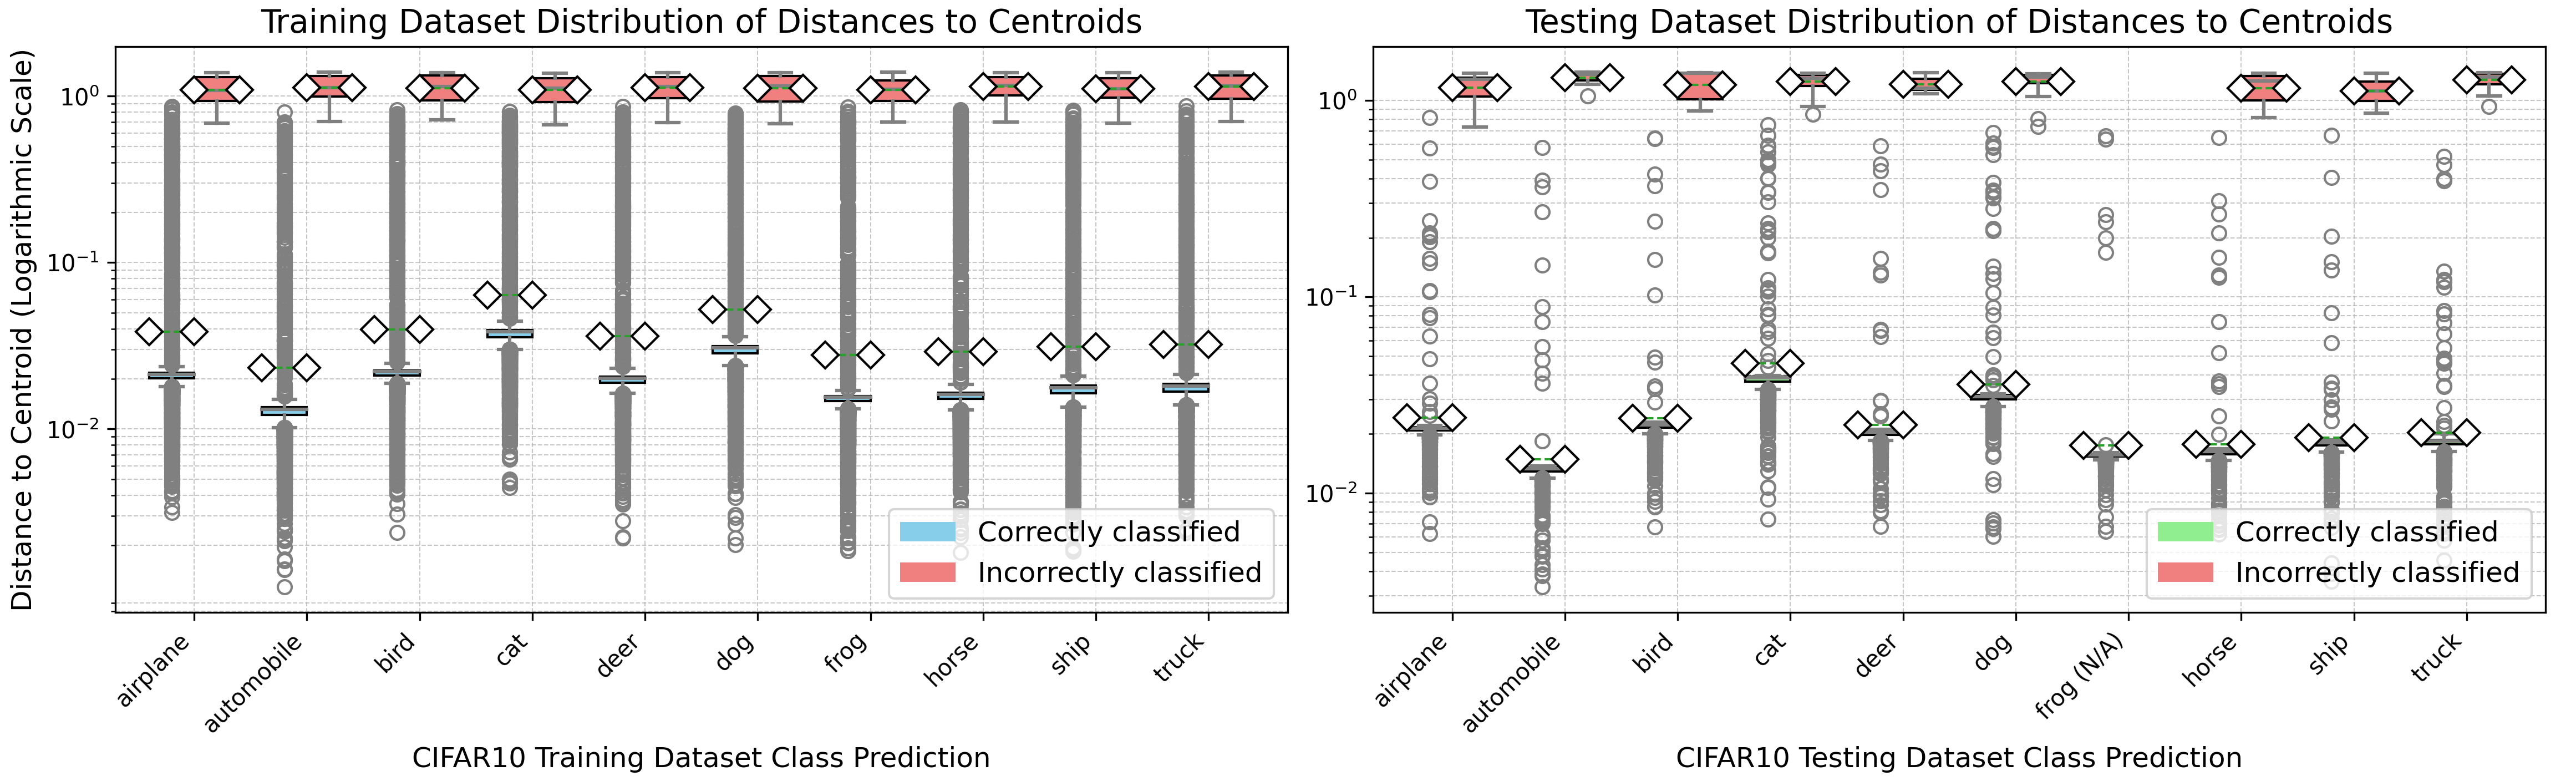
\includegraphics[width=0.99\textwidth]{Figures/CIFAR10_boxplots_side_by_side_x2.png}   \captionsetup{justification=raggedright,singlelinecheck=false}
    \caption{Distribution of Distances to Centroids for Correctly and Incorrectly Classified Instances in Training and Testing CIFAR-10 data, where training data is on the left and testing data is displayed on the right. Distances on y axis are shown on a logarithmic scale. Centroids are obtained from correctly classified training examples, then used for both training and testing datasets, a cluster is not created from the testing softmax distances. On the testing dataset, no frogs as misclassified, hence the missing top bloxplot. The corresponding plot for the MNIST dataset results is given in the supplementary materials.}
    \label{fig:CIFAR10_boxplots_side_by_side_x2}
\end{figure*}

% MNIST CNN

\textbf{Convolutional Neural Network}: A Convolutional Neural Network (CNN) is used to classify handwritten digits from the MNIST dataset, consisting of 60,000 training images and 10,000 testing images, each of size 28x28 grayscale (single channel) pixels, representing digits from 0 to 9.

The CNN architecture, implemented using PyTorch, consists of two convolutional layers followed by two fully connected layers. The first convolutional layer has 16 filters with a kernel size of 3x3 and a padding of 1. The second convolutional layer has 32 filters with the same kernel size and padding. Each convolutional layer is followed by a ReLU activation function and a max-pooling layer with a pool size of 2x2. The output of the second convolutional layer is flattened and passed through two fully connected layers with 128 and 10 neurons, respectively. The final output is passed through a log-softmax function to obtain the predicted class probabilities.
\begin{algorithm}
\caption{Find Minimum Softmax Distances to Centroids for Incorrectly Predicted Digits (Threshold)}
\label{alg:min_distance} 
\begin{algorithmic}[1]
\Procedure{FindMinDistances}{$data$}
    \State $labels \gets [0, 1, 2, 3, 4, 5, 6, 7, 8, 9]$
    \State $thresh \gets \text{empty array of shape } (10, 2)$
    \For{$i \gets 0 \text{ to } 9$}
        \State $label \gets labels[i]$
        \State $min\_dist \gets \min(data[data[:, 1] == label, 0])$
        \State $thresh[i, 0] \gets min\_dist$
        \State $thresh[i, 1] \gets label$
    \EndFor
    \State \textbf{return} $thresh$
\EndProcedure
\end{algorithmic}
\end{algorithm}
The model was trained using the Stochastic Gradient Descent (SGD) optimizer with a learning rate of 0.01 and a batch size of 64. The learning rate was determined using a custom learning rate function that decreases the learning rate over time. The Cross-Entropy Loss function was used as the criterion for optimization. The model was trained for 10 epochs.

The MNIST dataset was preprocessed using a transformation pipeline that converted the images to PyTorch tensors and normalized the pixel values to have a mean of 0.5 and a standard deviation of 0.5. The dataset was then loaded using PyTorch's DataLoader, for batch processing and shuffling of the data.

The total number of parameters for the MNIST classification CNN is 206,922 and took 5m6s to train on a Dell Precision Tower 5810 with a 6 core Intel Xeon Processor and 32GB memory running Ubuntu 18.04.  
%%%%%%%%%%%%%%%%%%%%
% NETWORK TRAINING %
%%%%%%%%%%%%%%%%%%%%
% Training time
The CNN/MNIST classifier took 5m6s to train. The accuracy on the training dataset is 98.38\% and 98.46\% on the testing dataset. 


\textbf{Vision Transformer}: The Vision Transformer (ViT) architecture \cite{dosovitskiy2020image} is implemented using the Hugging Face Transformers \cite{wolf2020huggingfaces}
library. The model used in this study, 'google/vit-base-patch16-224-in21k' \cite{wu2020visual}, is pre-trained on the ImageNet-21k dataset \cite{deng2009imagenet}, which contains 14 million labeled images. The pre-trained model is then fine-tuned on the CIFAR-10 dataset.
The ViT model divides an input image into patches and processes them using a Transformer encoder. The model used in this study has a patch size of 16x16 and an image size of 224x224. The ViT model outputs a representation of the image, which is then passed through a linear layer to obtain the final class probabilities.
The model has 86.4M parameters and is fine-tuned to classify images from the CIFAR-10 dataset, consisting of 50,000 training images and 10,000 testing images, each of size 32x32 pixels, representing 10 different classes: airplane, automobile, bird, cat, deer, dog, frog, horse, ship, and truck.

The data preprocessing pipeline involves on-the-fly data augmentation using the torchvision library's transforms module. The training data undergoes random resized cropping, random horizontal flipping, conversion to a tensor, and normalization. The validation and testing data are resized, center-cropped, converted to a tensor, and normalized.

The model is trained using the Hugging Face Trainer API. The learning rate is set to $2 \times 10^{-5}$, the per-device train batch size is 10, the per-device eval batch size is 4, and the number of training epochs is 3. The weight decay is set to 0.01. The model is trained on Google Colab Pro, T4 GPU hardware accelerator with high ram. The ViT/CIFAR-10 classifier took 1h15m to train, registering 99.04\% accuracy on the testing dataset.

% Moved from Results for a better spread of images

\begin{figure*}[ht]
    \centering
    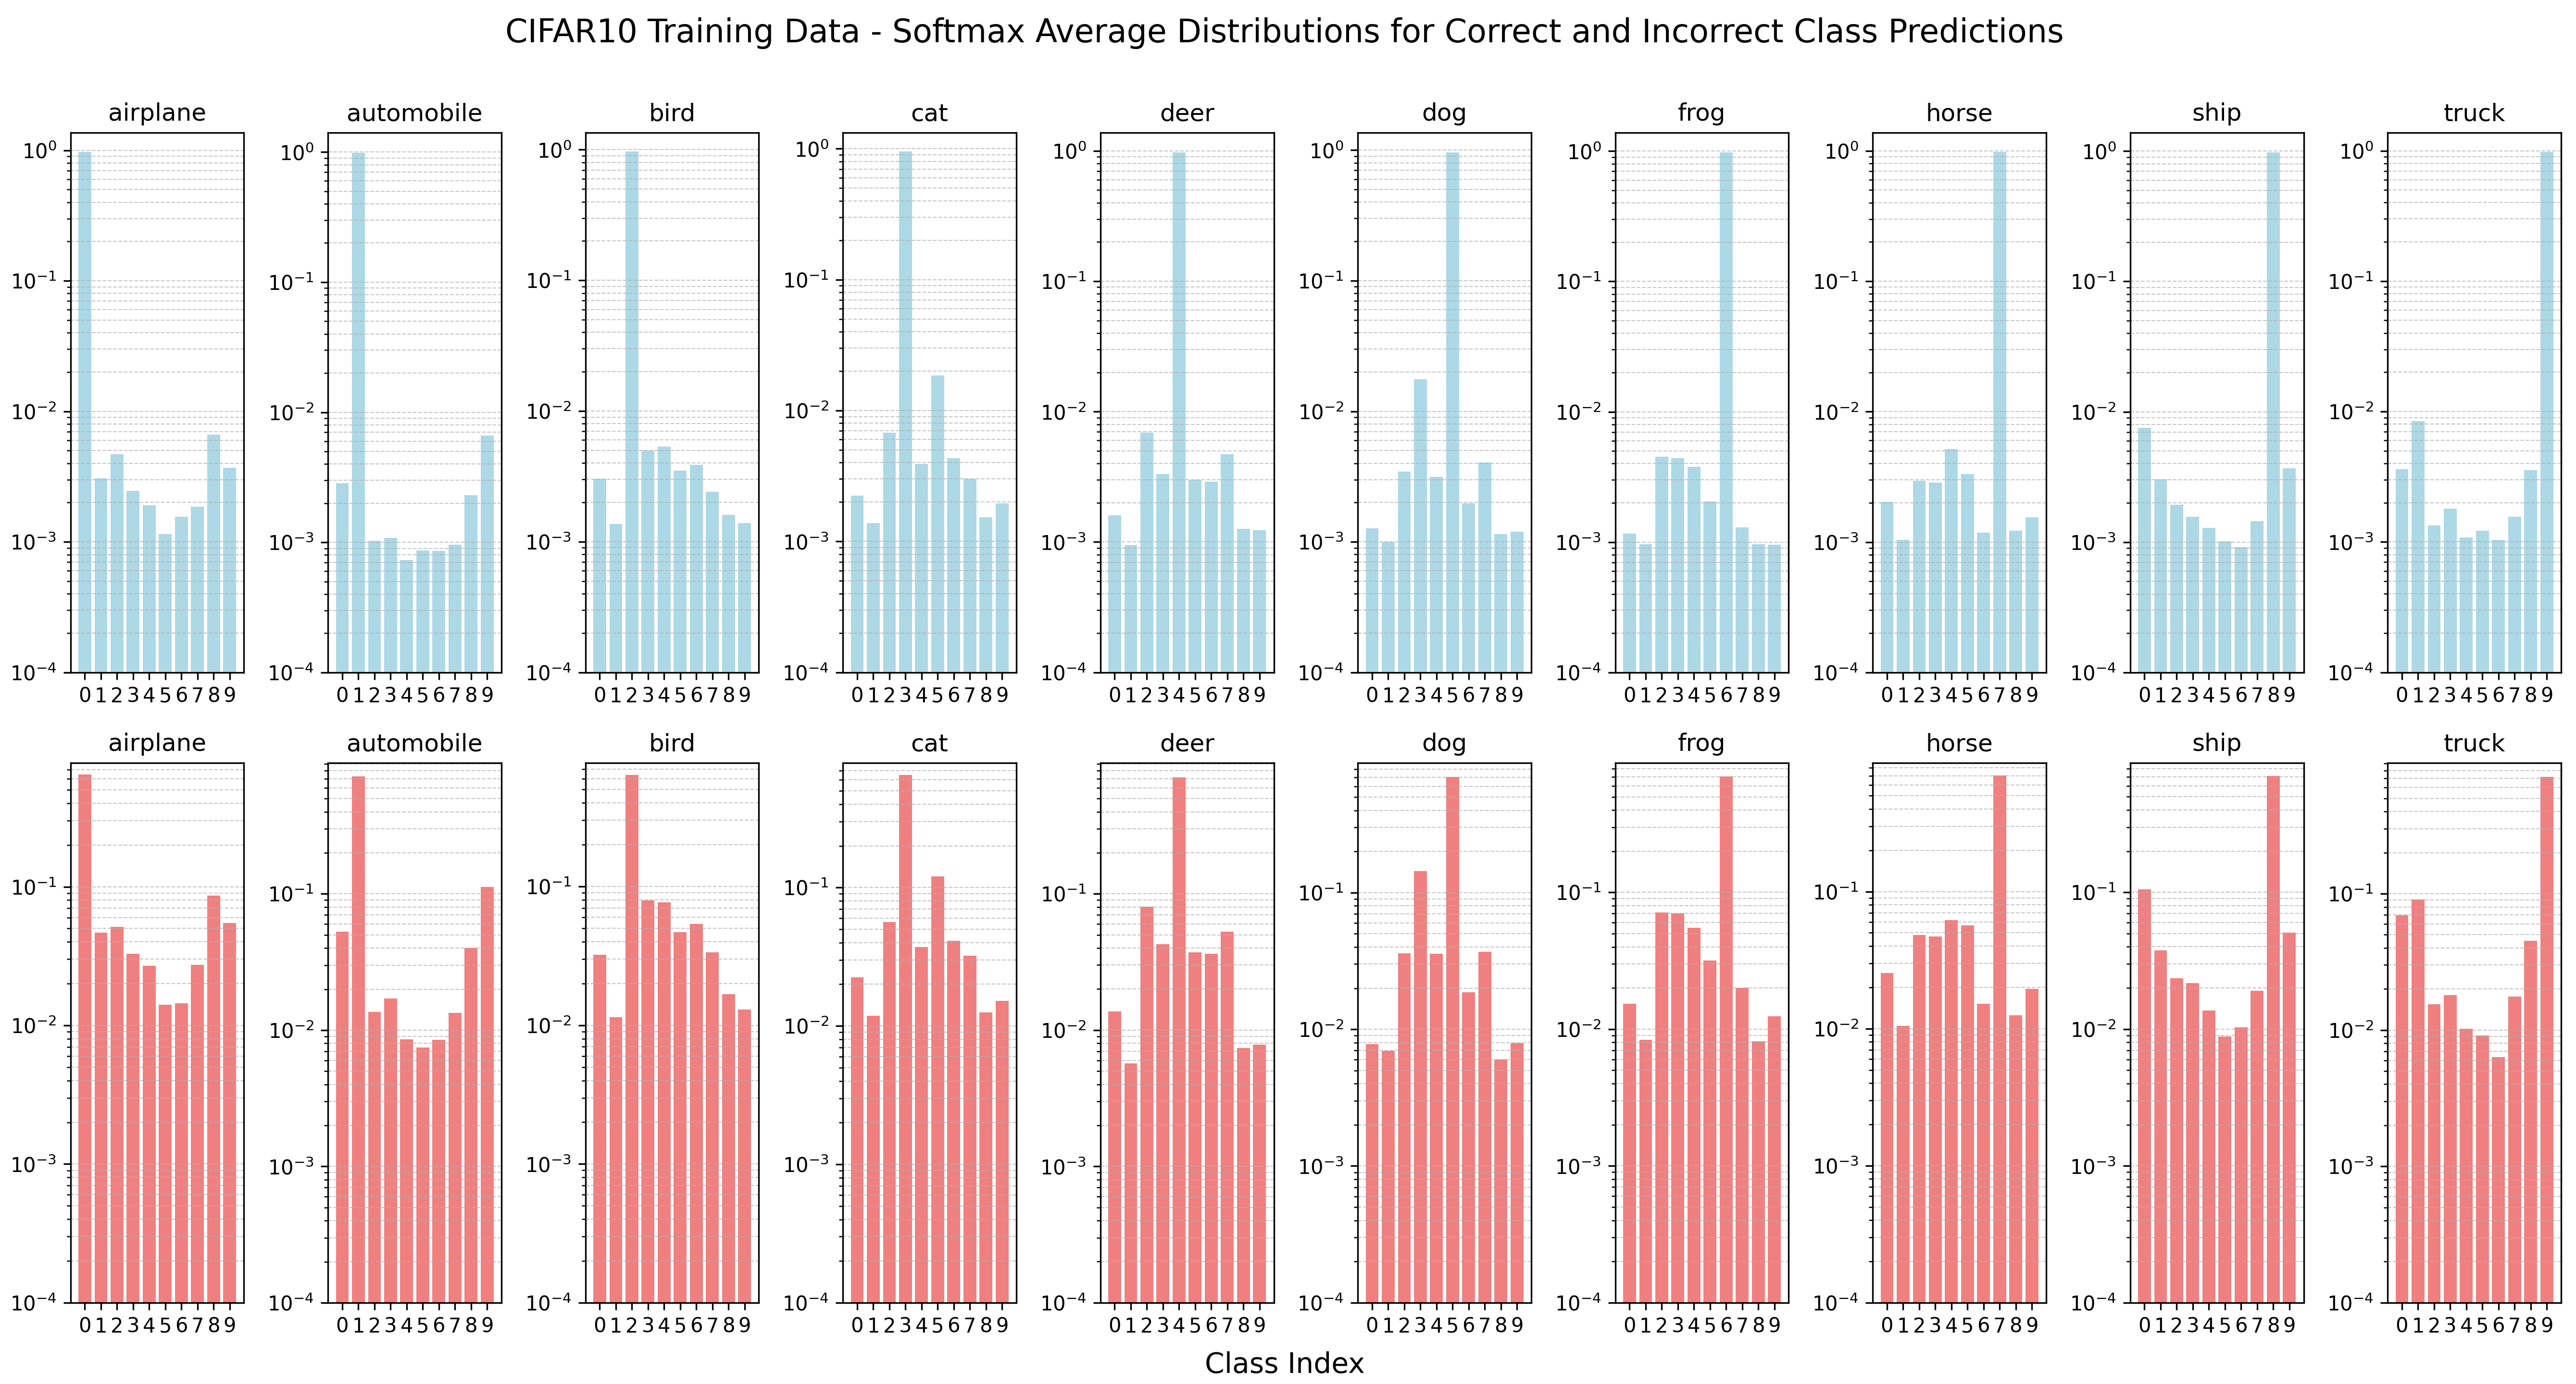
\includegraphics[width=0.99\textwidth]{Figures/CIFAR10_training_plot_centroid_distance_bars.png}
    \caption{Average Softmax Probabilities for ViT Correctly and Incorrectly Classified Classes in the CIFAR-10 Training Dataset. The ViT/CIFAR-10 testing dataset, and CNN/MNIST training and testing dataset equivalent results are given in the supplementary materials.}
    \label{fig:CIFAR10_training_plot_centroid_distance_bars.png}
\end{figure*}
%%%%%%%%%%%
% RESULTS %
%%%%%%%%%%%

\section{Experimental Results and Discussion}

In this section, we present and discuss our results for CIFAR-10/ViT and MNIST/CNN. 
%%%%%%%%%%%%%%%%%%%%%%%%%%%%%%%%%%%%%
% CIFAR10 MNIST SOFTMAX DISTANCE TO %
% CLUSTER CENTROID STATISTICS       %
%%%%%%%%%%%%%%%%%%%%%%%%%%%%%%%%%%%%%

\begin{table*}[ht]
\centering
\begin{tabular}{c|cccccc|cccccc}
\hline
& \multicolumn{6}{c|}{Training Dataset Correct Predictions} & \multicolumn{6}{c}{Training Dataset Incorrect Predictions} \\
Digit & Mean & Median & Min & Max & $\sigma$ & Count & Mean & Median & Min & Max & $\sigma$ & Count \\ \hline
0 & 0.0166 & 0.0088 & 0.0018 & \textbf{0.8433} & 0.0536 & 5890 & 0.9955 & 0.9552 & \textbf{0.7037} & 1.3681 & 0.1756 & 33 \\
1 & 0.0154 & 0.0085 & 0.0020 & \textbf{0.7051} & 0.0486 & 6704 & 1.0912 & 1.0771 & \textbf{0.7247} & 1.3909 & 0.2197 & 38 \\
2 & 0.0370 & 0.0208 & 0.0056 & \textbf{0.7453} & 0.0746 & 5859 & 1.0409 & 1.0460 & \textbf{0.6962} & 1.3912 & 0.2064 & 99 \\
3 & 0.0352 & 0.0192 & 0.0055 & \textbf{0.7509} & 0.0754 & 6019 & 1.0522 & 1.0338 & \textbf{0.7139} & 1.3999 & 0.2143 & 112 \\
4 & 0.0295 & 0.0166 & 0.0031 & \textbf{0.6933} & 0.0661 & 5755 & 1.0681 & 1.0642 & \textbf{0.7139} & 1.4010 & 0.2045 & 87 \\
5 & 0.0298 & 0.0165 & 0.0024 & \textbf{0.7634} & 0.0693 & 5339 & 1.0572 & 1.0560 & \textbf{0.7066} & 1.3956 & 0.2000 & 82 \\
6 & 0.0154 & 0.0081 & 0.0015 & \textbf{0.7981} & 0.0485 & 5884 & 1.0485 & 1.0702 & \textbf{0.7068} & 1.4015 & 0.2110 & 34 \\
7 & 0.0302 & 0.0171 & 0.0028 & \textbf{0.7365} & 0.0678 & 6199 & 1.0133 & 0.9764 & \textbf{0.6960} & 1.3989 & 0.2160 & 66 \\
8 & 0.0619 & 0.0363 & 0.0092 & \textbf{0.7788} & 0.0989 & 5581 & 1.0232 & 1.0083 & \textbf{0.6852} & 1.3816 & 0.1990 & 270 \\
9 & 0.0399 & 0.0232 & 0.0048 & \textbf{0.7616} & 0.0781 & 5844 & 1.0576 & 1.0830 & \textbf{0.7179} & 1.3974 & 0.2201 & 105 \\ \hline
& \multicolumn{6}{c|}{Testing Dataset Correct Predictions} & \multicolumn{6}{c}{Testing Dataset Incorrect Predictions} \\
Digit & Mean & Median & Min & Max & $\sigma$ & Count & Mean & Median & Min & Max & $\sigma$ & Count \\ \hline
0 & 0.0141 & 0.0075 & 0.0021 & \textbf{0.7225} & 0.0506 & 977 & 1.0329 & 1.0185 & \textbf{0.7923} & 1.2880 & 0.2026 & 3 \\
1 & 0.0126 & 0.0071 & 0.0023 & \textbf{0.6737} & 0.0445 & 1129 & 0.9823 & 0.9556 & \textbf{0.7278} & 1.2445 & 0.1898 & 6 \\
2 & 0.0354 & 0.0202 & 0.0037 & \textbf{0.6697} & 0.0704 & 1015 & 1.0855 & 1.0725 & \textbf{0.7010} & 1.3833 & 0.1844 & 17 \\
3 & 0.0331 & 0.0177 & 0.0049 & \textbf{0.7515} & 0.0765 & 998 & 0.9823 & 0.9752 & \textbf{0.7102} & 1.3230 & 0.2044 & 12 \\
4 & 0.0306 & 0.0169 & 0.0047 & \textbf{0.6603} & 0.0678 & 972 & 0.9309 & 0.8725 & \textbf{0.7073} & 1.3110 & 0.1923 & 10 \\
5 & 0.0313 & 0.0173 & 0.0051 & \textbf{0.6324} & 0.0692 & 883 & 1.1874 & 1.2976 & \textbf{0.8477} & 1.3982 & 0.2067 & 9 \\
6 & 0.0172 & 0.0088 & 0.0029 & \textbf{0.7135} & 0.0545 & 941 & 1.0737 & 1.0242 & \textbf{0.7240} & 1.4009 & 0.2120 & 17 \\
7 & 0.0295 & 0.0165 & 0.0036 & \textbf{0.6939} & 0.0678 & 1009 & 0.9665 & 0.8833 & \textbf{0.7148} & 1.3628 & 0.2016 & 19 \\
8 & 0.0616 & 0.0372 & 0.0114 & \textbf{0.7328} & 0.0918 & 934 & 1.0513 & 1.0399 & \textbf{0.7252} & 1.3842 & 0.2022 & 40 \\
9 & 0.0359 & 0.0206 & 0.0042 & \textbf{0.6870} & 0.0765 & 980 & 1.0502 & 1.0486 & \textbf{0.6968} & 1.3838 & 0.2197 & 29 \\ \hline
\end{tabular}
\captionsetup{justification=raggedright,singlelinecheck=false}
\caption{Statistical Summary of MNIST Softmax Output Distances to Centroids for Different Datasets and Prediction Outcomes. The centroids are obtained from Softmax outputs for correct class predictions from the training dataset.}
\label{tab:distance_to_centroid}
\end{table*}

% DATA for table above
%        Mean    Median       Min       Max  Standard Deviation  Count
% 0  0.016608  0.008843  0.001769  0.843304            0.053614   5890
% 1  0.015435  0.008516  0.002036  0.705149            0.048557   6704
% 2  0.036996  0.020828  0.005605  0.745250            0.074615   5859
% 3  0.035151  0.019205  0.005478  0.750860            0.075377   6019
% 4  0.029493  0.016613  0.003111  0.693346            0.066094   5755
% 5  0.029819  0.016509  0.002448  0.763396            0.069287   5339
% 6  0.015405  0.008078  0.001526  0.798075            0.048491   5884
% 7  0.030247  0.017138  0.002791  0.736508            0.067780   6199
% 8  0.061884  0.036283  0.009184  0.778795            0.098932   5581
% 9  0.039943  0.023188  0.004768  0.761636            0.078053   5844
%        Mean    Median       Min       Max  Standard Deviation  Count
% 0  0.995516  0.955230  0.703653  1.368133            0.175639     33
% 1  1.091157  1.077065  0.724706  1.390934            0.219724     38
% 2  1.040888  1.046023  0.696177  1.391211            0.206378     99
% 3  1.052159  1.033801  0.713948  1.399858            0.214313    112
% 4  1.068138  1.064157  0.713896  1.400997            0.204490     87
% 5  1.057245  1.055964  0.706555  1.395563            0.200003     82
% 6  1.048483  1.070162  0.706828  1.401450            0.211018     34
% 7  1.013332  0.976427  0.695997  1.398902            0.216013     66
% 8  1.023217  1.008262  0.685179  1.381630            0.199017    270
% 9  1.057626  1.082991  0.717850  1.397425            0.220102    105
%        Mean    Median       Min       Max  Standard Deviation  Count
% 0  0.014064  0.007518  0.002131  0.722502            0.050551    977
% 1  0.012627  0.007062  0.002254  0.673694            0.044504   1129
% 2  0.035369  0.020174  0.003719  0.669724            0.070428   1015
% 3  0.033119  0.017744  0.004876  0.751473            0.076455    998
% 4  0.030573  0.016858  0.004709  0.660308            0.067756    972
% 5  0.031271  0.017275  0.005053  0.632375            0.069207    883
% 6  0.017175  0.008774  0.002851  0.713528            0.054455    941
% 7  0.029476  0.016466  0.003639  0.693906            0.067756   1009
% 8  0.061609  0.037214  0.011389  0.732832            0.091848    934
% 9  0.035850  0.020602  0.004236  0.686980            0.076507    980
%        Mean    Median       Min       Max  Standard Deviation  Count
% 0  1.032918  1.018475  0.792297  1.287982            0.202620      3
% 1  0.982310  0.955644  0.727825  1.244521            0.189784      6
% 2  1.085502  1.072510  0.700976  1.383269            0.184444     17
% 3  0.982309  0.975231  0.710249  1.322951            0.204446     12
% 4  0.930852  0.872484  0.707302  1.310962            0.192325     10
% 5  1.187412  1.297633  0.847685  1.398223            0.206653      9
% 6  1.073695  1.024168  0.724028  1.400876            0.211957     17
% 7  0.966459  0.883283  0.714793  1.362762            0.201621     19
% 8  1.051282  1.039866  0.725232  1.384221            0.202232     40
% 9  1.050175  1.048609  0.696760  1.383811            0.219746     29

%\subsection{Softmax Distance to Class Centroid Statistics}
% Discussion about table results
\noindent \textbf{Softmax Distance to Class Centroid Statistics:} We store the softmax outputs, true and predicted labels for the MNIST and CIFAR-10 training datasets, we obtain the mean values for all correctly predicted classes, use the values in algorithm \ref{alg:k-means-centroid-init}  to initialise the cluster centroids, then using the procedure described in algorithm \ref{alg:min_distance} and the same hardware used to train the MNIST classifier CNN, generate K-Means clusters and compute statistics as presented in Table \ref{tab:distance_to_centroid} (for the MNIST results), a summary of the distances between the softmax outputs of a model and the centroids for each digit class (0-9) in the MNIST dataset. The centroids are calculated using the softmax outputs for correct predictions from the training dataset. The table is divided into four main sections: Training Dataset Correct Predictions, Training Dataset Incorrect Predictions, Testing Dataset Correct Predictions, and Testing Dataset Incorrect Predictions. For each digit and section, statistics are displayed with respect to softmax distance from each class to its centroid: the mean, median, minimum (highlighted in bold for the testing datasets), maximum (highlighted in bold for the training datasets), standard deviation ($\sigma$), and count of instances are provided. We note that for the correct predictions, the mean softmax distance to class centroid for digits zero, one and six are lowest (network prediction accuracy is high) while for digit 8 the mean softmax distance to class centroid is a comparatively larger value (netrowk prediction accuracy is not as high). The significance of the bold highlight for Max values in the Training section, and Min values in the Correct Prediction sections, is that the Min values in the Incorrect Predictions sections, is that the latter is effectively the Threshold we propose be used as a boundary for accepting the class prediction as accurate. Anything softmax distances equal or above the threshold will be considered not safe to use. It becomes evident by comparing both columns, that for the training dataset, there is a significant overlap between Max and Min columns, however, the testing dataset presents an interesting property in that there is less of an overlap. The significance of the overlap is that any correct predictions within the overlap will be tagged as unsafe, for the scheme we propose to hold, which means more manual classification and human intervention on the downside, and on the upside a high likelihood that every prediction with softmax distance below the threshold is accurate.

In practice a small number of samples, 0.04\%, consistent across both CIFAR-10 and MNIST testing dataset prediction, are found in the overlap, as shown later in Tables \ref{tab:centroid_distance_overlap_mnist} and \ref{tab:centroid_distance_overlap}. Also shown in Table \ref{tab:distance_to_centroid} are the softmax distance standard deviations and counts for correct and incorrect classifications.

%\subsection{Predictive Accuracy and Softmax Distance to Class Centroid}

\noindent \textbf{Predictive Accuracy and Softmax Distance to Class Centroid:} The confusion matrices in Figure \ref{fig:mnist_training_confusion_matrix} provide some insights into what are the most likely MNIST misclassifications at training time. We note that number zero is the digit less likely, and number eight is the digit most likely to be misclassified. Other digits that are less likely to be misclassified are digits one and; six in the training dataset, and five in the testing dataset. Digit eight is likely to be misclassified as six or nine, while digit three is likely to be misclassified as two, five or nine.

%%%%%%%%%%%%%%%%%%%%%%%%%%
% MNIST CONFUSION MATRIX %
%%%%%%%%%%%%%%%%%%%%%%%%%%

% plot produced with function call:
% conf_matrix1, conf_matrix2 = display_misclassifications_side_by_side_cifar10(train_np, test_np, 10, 11, class_labels, 20, 7, True)
% \begin{figure}[ht]
%     \centering
%     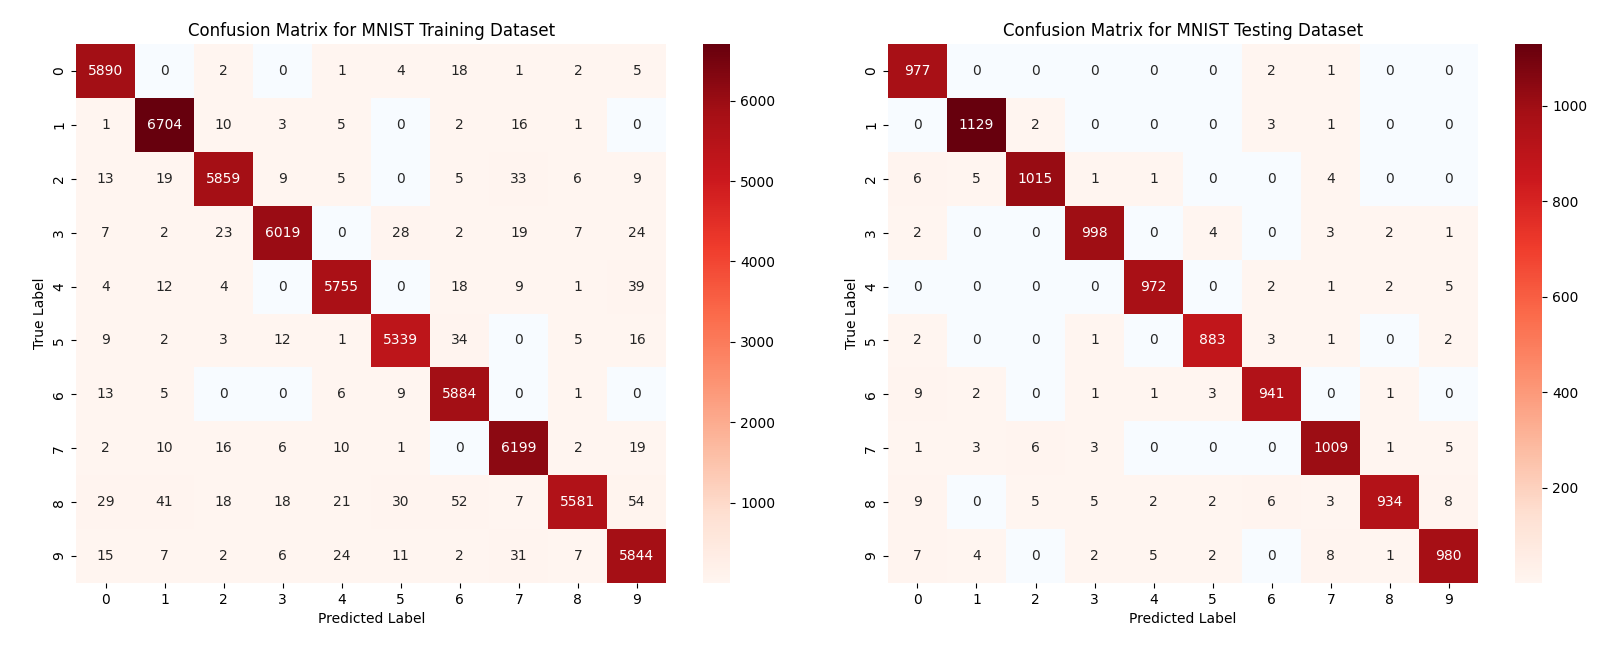
\includegraphics[width=0.99\columnwidth]{Figures/mnist_combined_confusion_matrix.png}
%     \caption{Please zoom in for detail. Confusion matrices for the MNIST classification model on the training dataset (left) and testing dataset (right). The matrices display the true labels on the vertical axis and the predicted labels on the horizontal axis. The diagonal elements represent correctly classified instances, while the off-diagonal elements indicate misclassifications.}
%     \label{fig:mnist_combined_confusion_matrix}
% \end{figure}

\begin{figure}[ht]
    \centering
    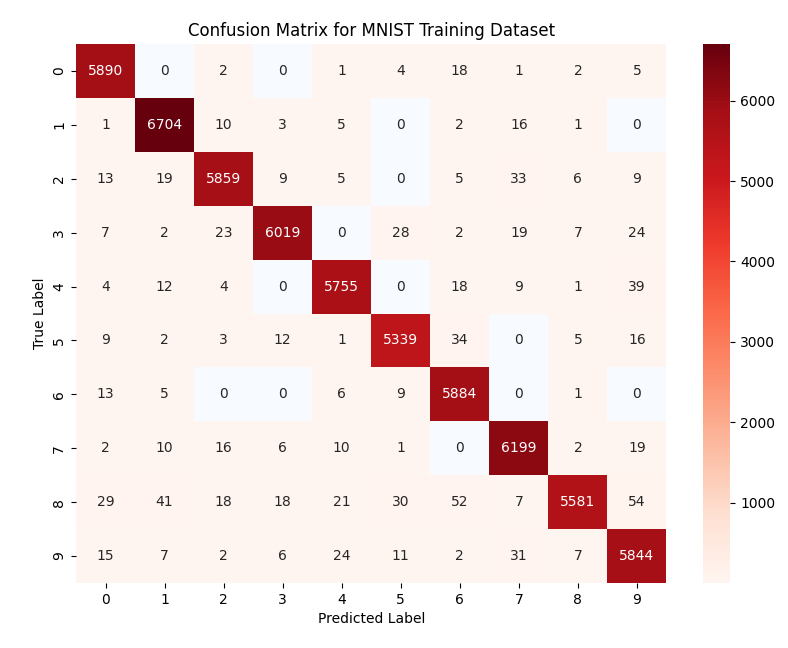
\includegraphics[width=0.99\columnwidth]{Figures/mnist_training_confusion_matrix.png}
    \caption{Confusion matrices for the MNIST classification model on the training dataset. The matrices display the true labels on the vertical axis and the predicted labels on the horizontal axis. The diagonal elements represent correctly classified instances, while the off-diagonal elements indicate misclassifications. The corresponding confusion matrix for the testing dataset is provided in the supplementary materials.}
    \label{fig:mnist_training_confusion_matrix}
\end{figure}

The confusion matrix for the CIFAR-10 training dataset in Figure \ref{fig:cifar10_training_confusion_matrix} illustrates the performance of a classifier model on the training dataset. For the training set, the model exhibits a strong diagonal, indicative of high classification accuracy for most classes. Nonetheless, certain classes show notable confusion, such as 'cat' with 'dog' and 'deer' with 'frog', and the confusion is reflected in the class softmax distance to cluster centroid.

Examining the testing dataset, the model achieves good classification success, with perfect recognition of 'frog' class. Misclassifications are present but considerably reduced compared to the training dataset, particularly for pairs such as 'truck' and 'automobile', as well as 'cat' and 'dog'. The reduced confusion in the test set is also reflected in the softmax distance to cluster centroid.

% plot produced with function call:
% conf_matrix1, conf_matrix2 = display_misclassifications_side_by_side_cifar10(train_np, test_np, 10, 11, class_labels, 20, 7, True)
\begin{figure}[ht]
    \centering   
    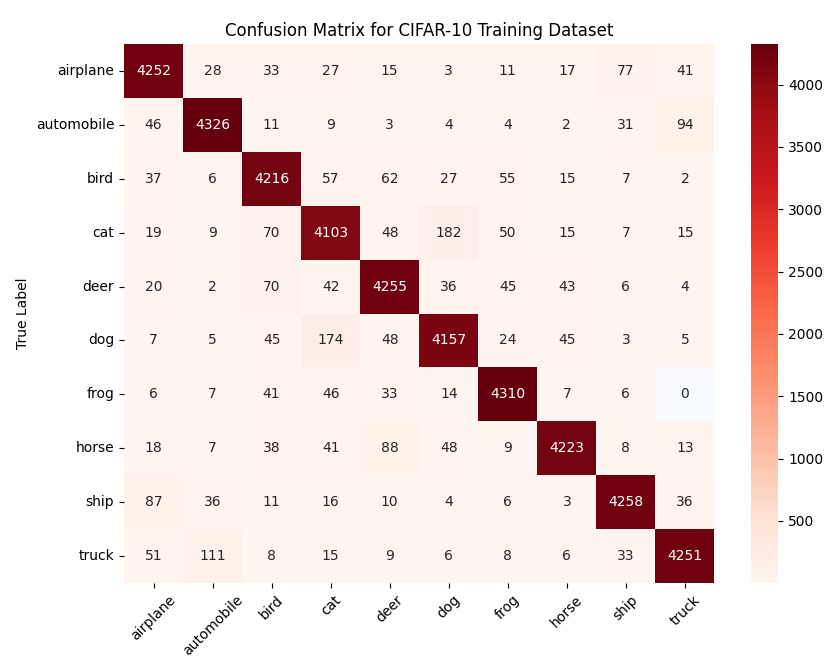
\includegraphics[width=0.99\columnwidth]{Figures/cifar10_training_confusion_matrix.png}
    \caption{Confusion matrix for the CIFAR-10 classifier model training dataset dataset dataset correct and incorrect classifications. The corresponding matrix for the testing dataset is given in the supplementary materials.}
    \label{fig:cifar10_training_confusion_matrix}
\end{figure}



%%%%%%%%%%%%%%%%%%%%%%%%%%%%%%%%%
% CIFAR10 BOXPLOTS SIDE BY SIDE %
%%%%%%%%%%%%%%%%%%%%%%%%%%%%%%%%%

%\subsection{Overlap between maximum and minimum softmax distances to class centroids}

% Figure \ref{fig:CIFAR10_boxplots_side_by_side_x2} presents box plots showing the distribution of distances to centroids for correctly and incorrectly classified instances in each class of the CIFAR-10 training and testing datasets.

% In the training dataset, the distances to centroids for correctly classified instances (green boxes) are generally lower than those for incorrectly classified instances (red boxes), indicating that correctly classified instances tend to be closer to their respective class centroids in the feature space. However, there is a small overlap between the distances of correctly and incorrectly classified instances, particularly in classes such as cat, dog, and deer. 

% The testing dataset exhibits a similar trend, with correctly classified instances having lower distances to centroids compared to incorrectly classified instances. The overlap between the two groups is less pronounced in the testing dataset, such as in classes like frog. This decreased overlap is expected, as the softmax distance to cluster centroids for incorrect classifications is larger, compared to training dataset. Note there is no frog boxplot for incorrect classifications, as reflected in the confusion matrix.

% The side-by-side boxplots convey the distributions of distances to centroids for both the training and testing sets, categorized by class. These distances are represented on a logarithmic scale, facilitating the visualization of a wide range of values. The boxplots are bifurcated into two sections for each class: correctly classified and incorrectly classified instances.

% For both the training and testing sets, there is a clear pattern where the correctly classified instances tend to have a smaller median distance to the class centroid compared to the incorrectly classified ones. This observation is consistent across all classes, suggesting that instances closer to the centroid of their respective class in the feature space are more likely to be classified correctly by the model. The notable overlap in the interquartile ranges, however, indicates that while distance to the centroid is an informative metric, it is not solely determinative of classification accuracy.

% The incorrectly classified instances exhibit greater variance in distances to the centroid, as evidenced by the longer whiskers and the presence of outliers. This variability implies that misclassified instances can sometimes be far off from the core cluster of their true class, potentially falling closer to the regions dominated by other classes in the feature space. This is indicative of boundary cases or instances that bear a resemblance to multiple categories.

% The consistency of these trends between the training and testing sets indicates that the distance to the centroid is a robust indicator of classification difficulty across the model’s application. The presence of some correctly classified instances at higher distances suggests that other factors also influence classification accuracy, such as the density of data points in the surrounding feature space, class overlap, or specific intra-class variabilities.

\noindent \textbf{Overlap between maximum and minimum softmax distances to class centroids:} Figure \ref{fig:CIFAR10_boxplots_side_by_side_x2} presents box plots showing the distribution of distances to centroids for correctly and incorrectly classified instances in each class of the CIFAR-10 training and testing datasets. In the training dataset, the distances to centroids for correctly classified instances (green boxes) are generally lower than those for incorrectly classified instances (red boxes), indicating that correctly classified instances tend to be closer to their respective class centroids in the feature space. However, there is a small overlap between the distances of correctly and incorrectly classified instances, particularly in classes such as cat, dog, and deer. The testing dataset exhibits a similar trend, with correctly classified instances having lower distances to centroids compared to incorrectly classified instances. The overlap between the two groups is less pronounced in the testing dataset, such as in classes like frog. Note there is no frog boxplot for incorrect classifications, as reflected in the confusion matrix.

% Moved to Methods to better spread out figures
% \begin{figure*}[ht]
%     \centering
%     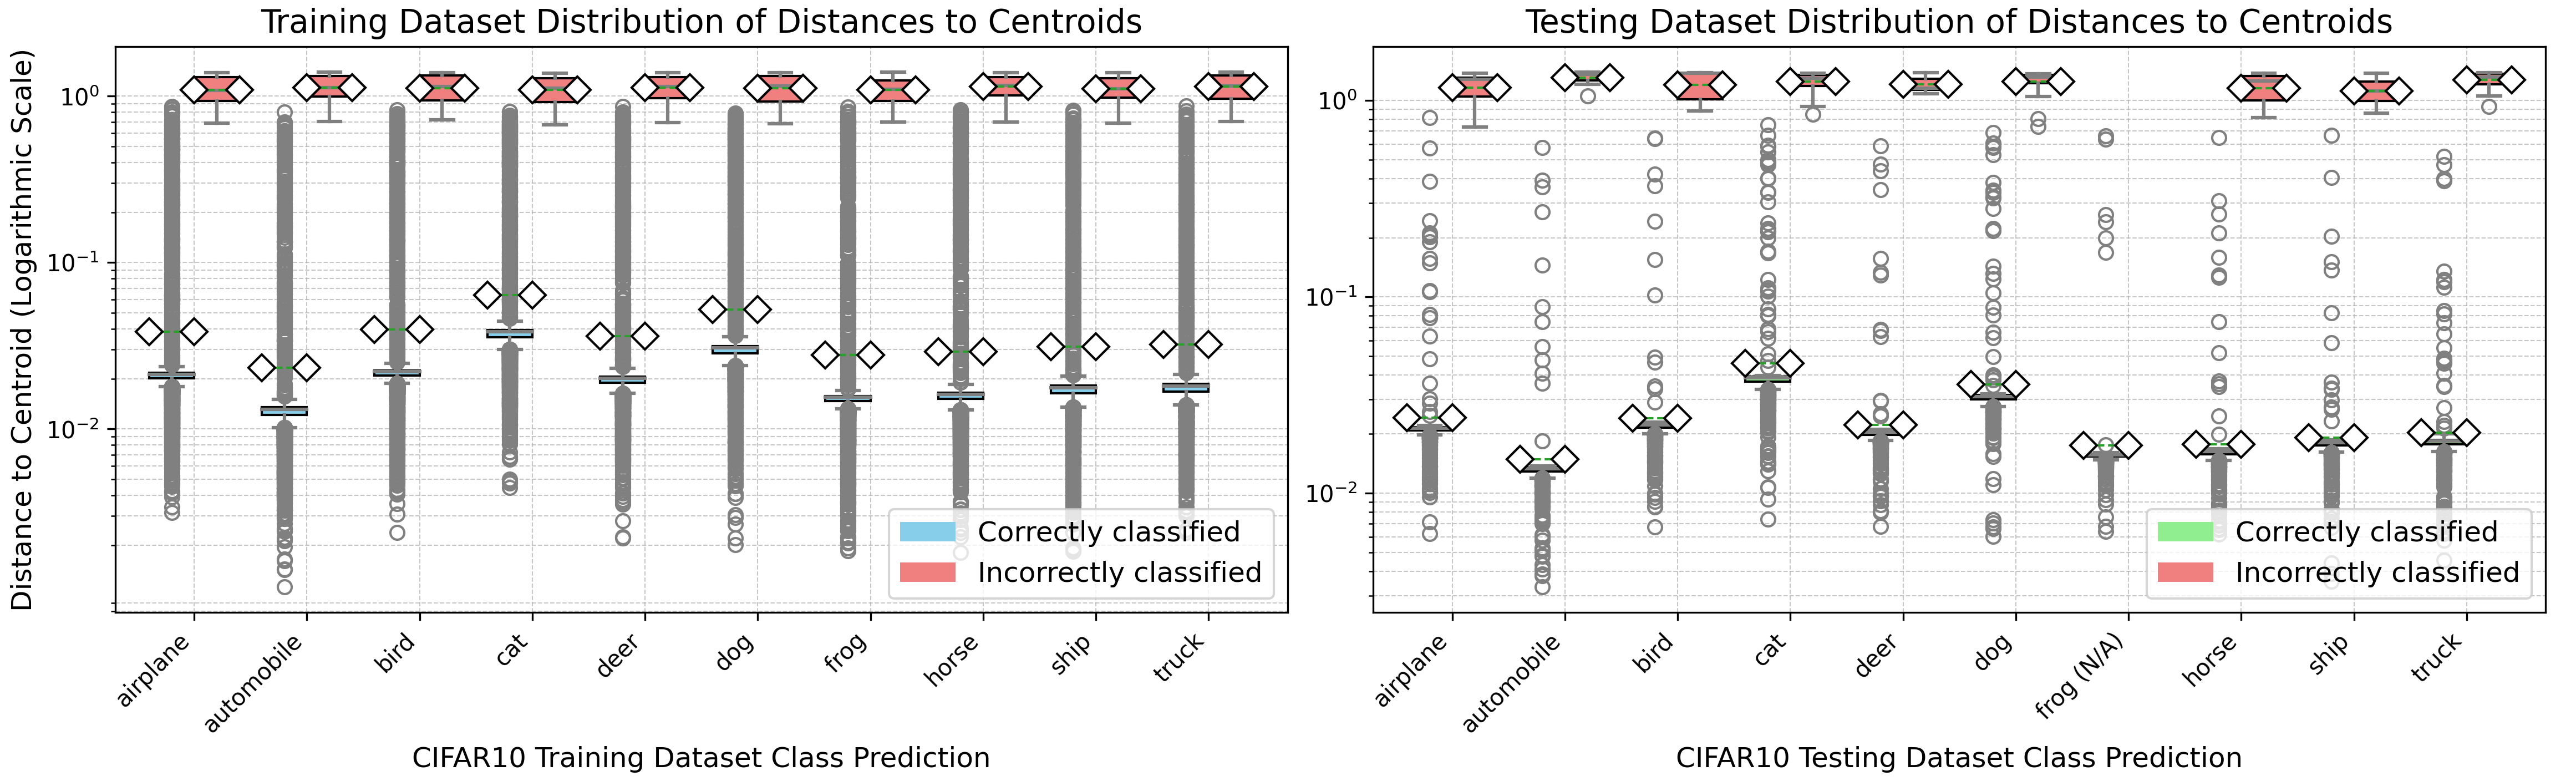
\includegraphics[width=0.99\textwidth]{Figures/CIFAR10_boxplots_side_by_side_x2.png}   \captionsetup{justification=raggedright,singlelinecheck=false}
%     \caption{Distribution of Distances to Centroids for Correctly and Incorrectly Classified Instances in Training and Testing CIFAR-10 data, where training data is on the left and testing data is displayed on the right. Distances on y axis are shown on a logarithmic scale. Centroids are obtained from correctly classified training examples, then used for both training and testing datasets, a cluster is not created from the testing softmax distances. On the testing dataset, no frogs as misclassified, hence the missing top bloxplot. The corresponding plot for the MNIST dataset results is given in the supplementary materials.}
%     \label{fig:CIFAR10_boxplots_side_by_side_x2}
% \end{figure*}

The side-by-side boxplots convey the distributions of distances to centroids for both the training and testing sets, categorized by class. These distances are represented on a logarithmic scale, facilitating the visualization of a wide range of values. For both sets, there is a clear pattern where the correctly classified instances tend to have a smaller median distance to the class centroid compared to the incorrectly classified ones. This observation is consistent across all classes, suggesting that instances closer to the centroid of their respective class in the feature space are more likely to be classified correctly by the model. The notable overlap in the interquartile ranges, however, indicates that while distance to the centroid is an informative metric, it is not solely determinative of classification accuracy.

The incorrectly classified instances exhibit greater variance in distances to the centroid, as evidenced by the longer whiskers and the presence of outliers. This variability implies that misclassified instances can sometimes be far off from the core cluster of their true class, potentially falling closer to the regions dominated by other classes in the feature space. This is indicative of boundary cases or instances that bear a resemblance to multiple categories. The consistency of these trends between the training and testing sets indicates that the distance to the centroid is a robust indicator of classification difficulty across the model's application. The presence of some correctly classified instances at higher distances suggests that other factors also influence classification accuracy, such as the density of data points in the surrounding feature space, class overlap, or specific intra-class variabilities.

% \subsection{Overlap table MNIST discussion 1}

%%%%%%%%%%%%%%%%%
% OVERLAP TABLE %
%%%%%%%%%%%%%%%%%

% Table generated with function call:
% centroid_distance_overlap_latex(d2c_train_correct, d2c_train_incorrect, d2c_test_correct, d2c_test_incorrect)
% \begin{table}[htbp]
% \centering
% \begin{tabular}{|c|c|c|c|c|c|c|}
% \hline
% Digit & \multicolumn{3}{c|}{Train Data - Train Centroids} & \multicolumn{3}{c|}{Test Data - Train Centroids} \\
% \hline
%  & Count & Total & Overlap & Count & Total & Overlap \\
% \hline
% 0 & 2 & 5890 & 0.03\% & 1 & 977 & 0.10\% \\
% 1 & 0 & 6704 & 0.00\% & 0 & 1129 & 0.00\% \\
% 2 & 1 & 5859 & 0.02\% & 0 & 1015 & 0.00\% \\
% 3 & 3 & 6019 & 0.05\% & 1 & 998 & 0.10\% \\
% 4 & 0 & 5755 & 0.00\% & 0 & 972 & 0.00\% \\
% 5 & 5 & 5339 & 0.09\% & 0 & 883 & 0.00\% \\
% 6 & 2 & 5884 & 0.03\% & 1 & 941 & 0.11\% \\
% 7 & 2 & 6199 & 0.03\% & 0 & 1009 & 0.00\% \\
% 8 & 12 & 5581 & 0.22\% & 1 & 934 & 0.11\% \\
% 9 & 1 & 5844 & 0.02\% & 0 & 980 & 0.00\% \\
% \hline
% Totals & 28 & 59074 & 0.05\% & 4 & 9838 & 0.04\% \\
% \hline
% \end{tabular}
% \caption{Counts of correctly classified training and testing image predictions with distance to centroids equal or above error threshold $\varepsilon_{\text{th}}(i)$ where $i$ is the digit class}
% \label{tab:centroid_distance_overlap_mnist}
% \end{table}

% Table \ref{tab:centroid_distance_overlap_mnist} show the counts of correctly classified training and testing examples that are assigned a  By choosing the $\varepsilon_{\text{th}}(i)$ the accuracy.

% The table presents an analysis of the counts and percentages of correctly classified images in the training and testing datasets that have softmax distances to their respective class centroids above a certain threshold. The threshold is determined by the nearest softmax distance to the centroid for the incorrectly classified classes.

% The table is divided into two main sections: "Train Data - Train Centroids" and "Test Data - Train Centroids." For each section, the table provides the count of images that satisfy the threshold condition, the total number of images in each class, and the percentage of overlap (i.e., the proportion of images above the threshold relative to the total count).

% Looking at the "Train Data - Train Centroids" section, we observe that the overlap percentages are relatively low, ranging from 0.00\% to 0.22\%. This suggests that only a small fraction of the correctly classified training images have softmax distances to their centroids above the threshold set by the incorrectly classified images. The highest overlap is observed for digit class 8, with 12 out of 5,581 images (0.22\%) having distances above the threshold.

% Similarly, in the "Test Data - Train Centroids" section, the overlap percentages are even lower, ranging from 0.00\% to 0.11\%. This indicates that the trained model is able to correctly classify the majority of the test images while maintaining a distance to the centroids below the threshold set by the incorrectly classified images. The highest overlap in the test data is observed for digit classes 6 and 8, with 1 out of 941 (0.11\%) and 1 out of 934 (0.11\%) images, respectively, having distances above the threshold.

% The "Totals" row summarizes the overall counts and overlap percentages across all digit classes. For the training data, 28 out of 59,074 images (0.05\%) have distances above the threshold, while for the test data, only 4 out of 9,838 images (0.04\%) exceed the threshold.

% These results suggest that the trained model is effective in correctly classifying images while maintaining a relatively small softmax distance to the class centroids. The low overlap percentages indicate that the majority of the correctly classified images are well-separated from the incorrectly classified images in terms of their softmax distances to the centroids. This analysis provides insights into the model's performance and its ability to distinguish between different digit classes based on the proximity of the images to their respective class centroids in the softmax space.


% The LaTeX table provides an overview of the distribution of correctly classified images for both the training and test datasets of a classification model applied to digit recognition. It compares the counts of images that have a softmax distance to centroid above a defined error threshold, \( \varepsilon_{\text{th}}(i) \), where \( i \) represents each digit class.

% The table is divided into two main sections: one for the training data using training centroids and the other for the test data also using training centroids. For each section, the table lists each digit from 0 to 9 and provides the count of images above the threshold, the total number of images in that digit class, and the percentage of overlap, which signifies the proportion of images above the threshold relative to the total count in that class.

% Notably, the 'Count' column for the training data shows very few images exceed the threshold for each digit, with '8' having the highest count at 12, while most other digits have counts of 5 or below. This suggests that the classification model is quite precise on the training data, with very few images being farther from the centroid than the threshold that demarcates incorrectly classified images. The 'Overlap' percentage supports this, with values being very low, the highest being only 0.22\% for digit '8'.

% For the test data, the counts of images above the threshold are even lower, with four out of the ten digits having a count of 1 and the rest having a count of 0. This indicates that the model generalizes well to unseen data, maintaining a low distance to centroid across the board for correctly classified images. The 'Overlap' percentages are in a similar range to the training data, with a 0.10\% overlap for digits '0' and '3', and a 0.11\% for digits '6' and '8'.

% In summary, the table suggests that the distance to the centroid can be a strong indicator of classification correctness, with the majority of correctly classified images lying closer to the centroid than the threshold set by the nearest incorrectly classified images. This behavior is consistent across both the training and test sets, with the test set showing a very similar or even slightly better distribution with respect to the threshold, which is indicative of good model generalization from training to testing. The very low overlap percentages suggest that the threshold is well-calibrated, capturing the distinction between correctly and incorrectly classified images effectively.


\noindent \textbf{Accuracy decrease vs threshold decrease:} Having observed that the percentage of correctly classified images that have softmax distances equal or above threshold is 0.04\% for both CIFAR-10 and MNIST testing datasets, we ask how lowering the threshold affects the accuracy. Figure \ref{fig:Combined_CIFAR10_MNIST_single_plot_accuracy_decrements.png} reveals that for MNIST (left plot) classes accurately classified by the CNN model, such as zero and one, even setting the threshold at 10\% of the original class thresholds (0.9 on the x axis), still present accuracies greater than 0.97, meaning the class clusters are tightly placed near the centroids, while for digit 8, the most misclassified digit, had the threshold been set at 10\% of the original value, the accuracy would expect to drop to 0.84, meaning 16\% of the predictions would be deferred to human judgement, and 84\% would be considered 100\% accurate..

Predictions with softmax distance to class centroid below the class threshold are expected to be 100\% accurate, class predictions with distances equal or greater than threshold are then left to human judgement.

% moved to appendix

%%%%%%%%%%%%%%%%%%%%%%%%%%%%%%%%%%%%%%%%%%%
% COMBINED CIFAR10 MNIST ACCURACY VS MEAN %
% CLASS PREDICTION DISTANCE TO THRESHOLD  %
%%%%%%%%%%%%%%%%%%%%%%%%%%%%%%%%%%%%%%%%%%%

% Plot created by joining plots created by plot_accuracy_vs_distance_linear_fit

% \begin{figure}[ht]
%     \centering
%     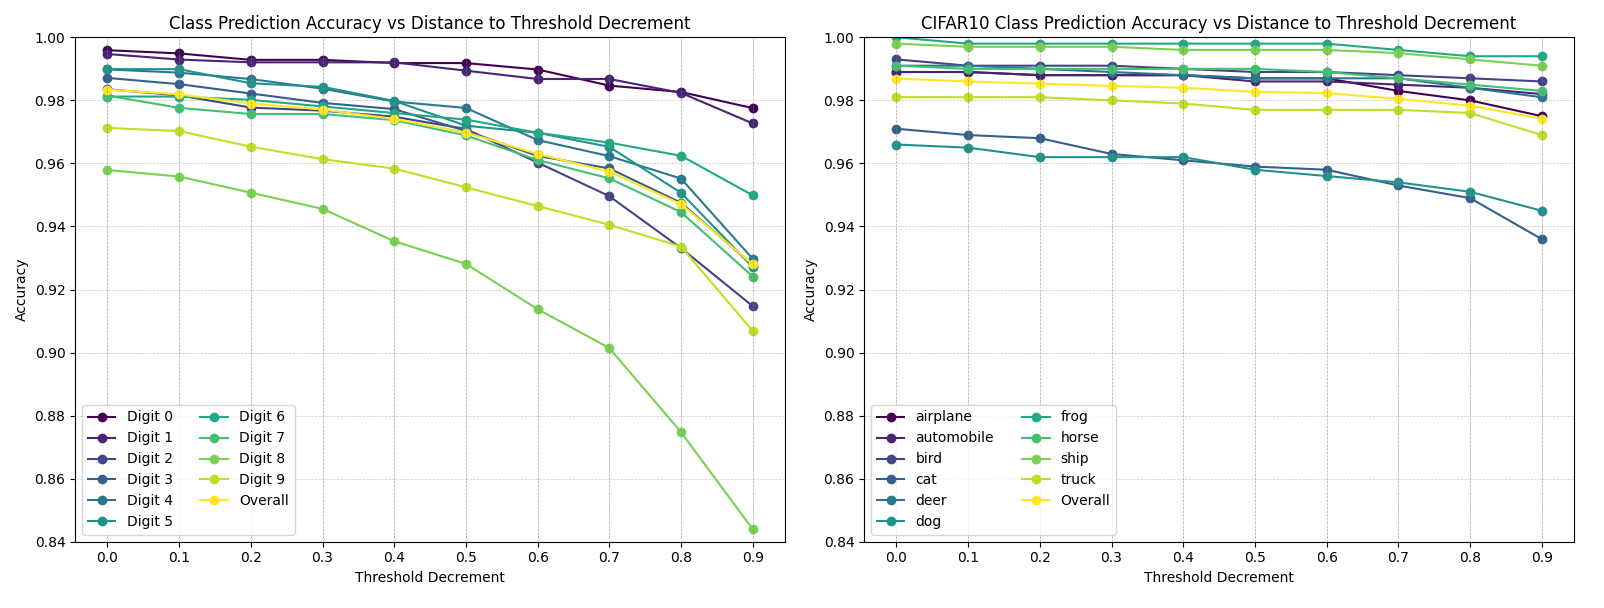
\includegraphics[width=0.99\columnwidth]{Figures/Combined_CIFAR10_MNIST_single_plot_accuracy_decrements.png}
%     \caption{Please zoom in for detail. Expected accuracy decrease as a result of threshold decrease. MNIST data is on the left, CIFAR-10 is on the right. The x axis shows the threshold decrement in factors of 0.1, that is, at 0.1 the threshold is 90\% of the original threshold while at 0.9 the threshold is 10\% of the original threshold and consequently neared to the class centroid.}
% \label{fig:Combined_CIFAR10_MNIST_single_plot_accuracy_decrements.png}
% \end{figure}

% moved to methods to spread out images
% % function call
% % plot_digit_averages(test_correct_predictions, test_incorrect_predictions, color1='lightgreen', color2='lightcoral', data="Testing Data")
% \begin{figure}[ht]
%     \centering
%     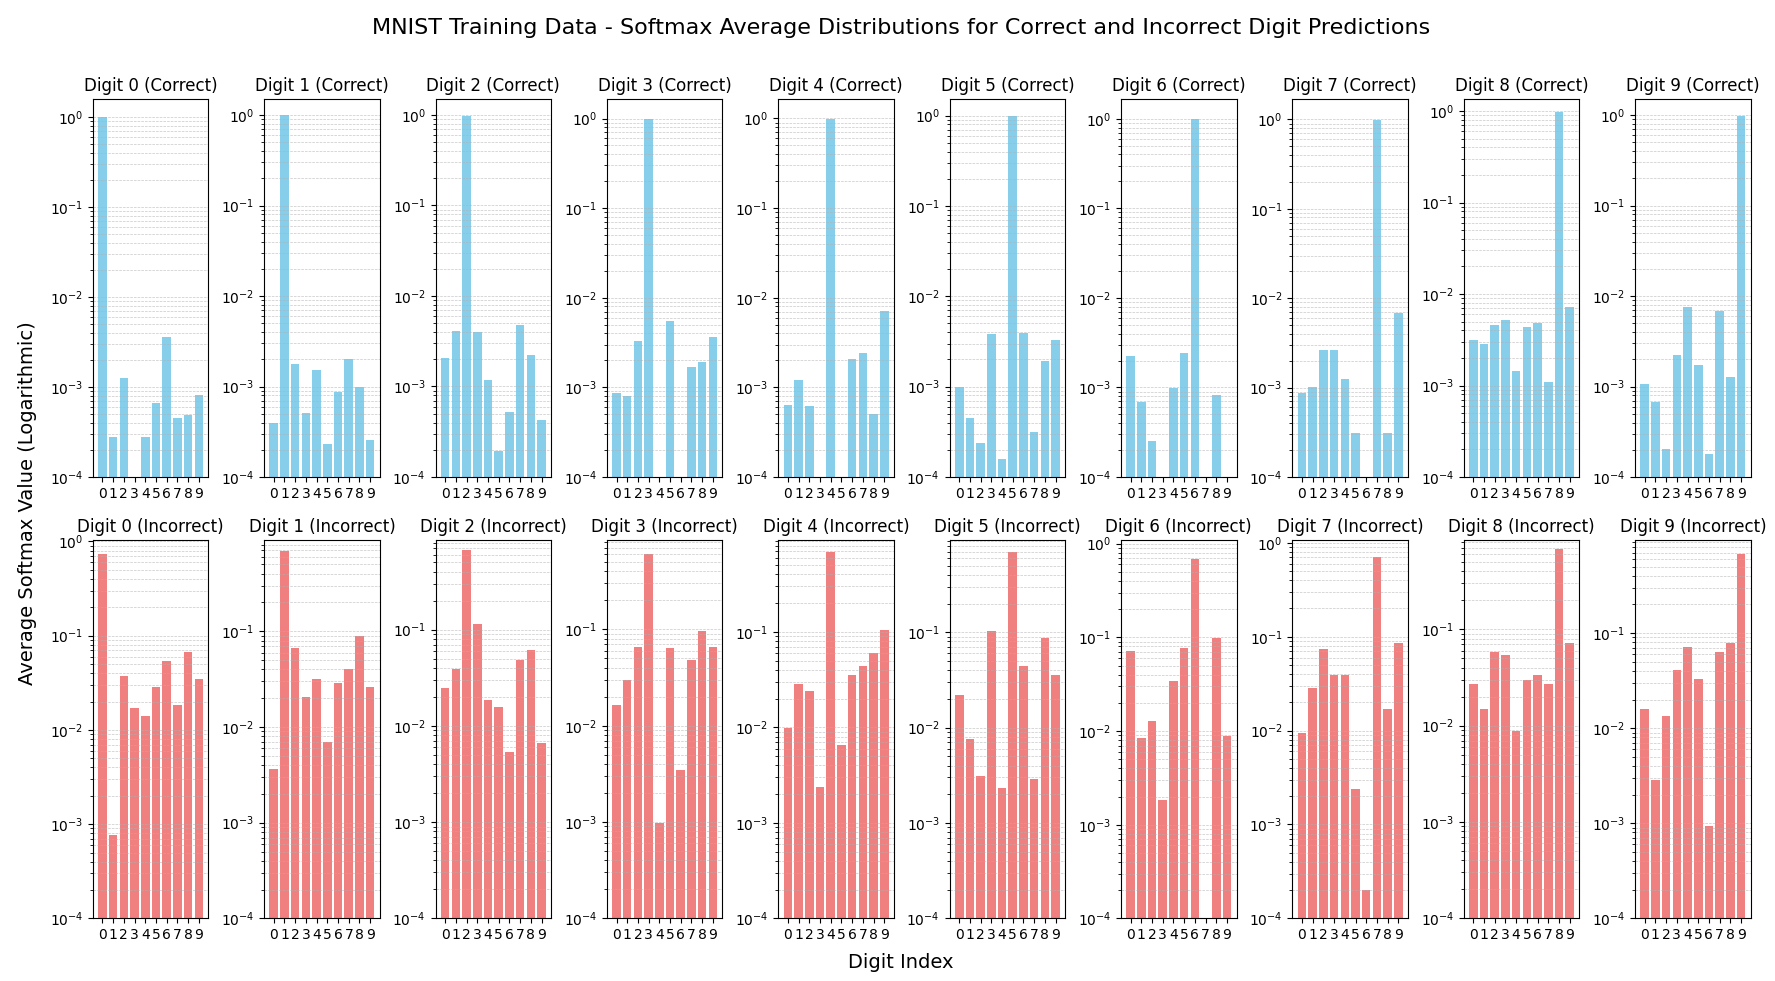
\includegraphics[width=0.99\columnwidth]{Figures/MNIST_Softmax_Averages_Training.png}
%     \caption{Please zoom in for detail. Average Softmax Probabilities for Correctly and Incorrectly Classified Digits in the MNIST Testing Dataset.}
%     \label{fig:MNIST_Softmax_Averages_Training}
% \end{figure}

% moved to appendix
% Figure \ref{fig:MNIST_Softmax_Averages_Training} shows the average softmax probabilities for each digit class (0 to 9) in the MNIST training dataset, separated into correctly classified instances (top row) and incorrectly classified instances (bottom row). The probabilities are displayed on a logarithmic scale. For correctly classified digits, the highest average probability is observed for the corresponding true digit class, indicating strong confidence in the correct predictions. In contrast, for incorrectly classified digits, the average probabilities are more evenly distributed across different digit classes, suggesting lower confidence and potential confusion between similar-looking digits.
% Figure \ref{fig:MNIST_Softmax_Averages_Testing} is the corresponding plot for the MNIST testing dataset.

% % function call
% % plot_digit_averages(test_correct_predictions, test_incorrect_predictions, color1='lightgreen', color2='lightcoral', data="Testing Data")
% \begin{figure}[ht]
%     \centering
%     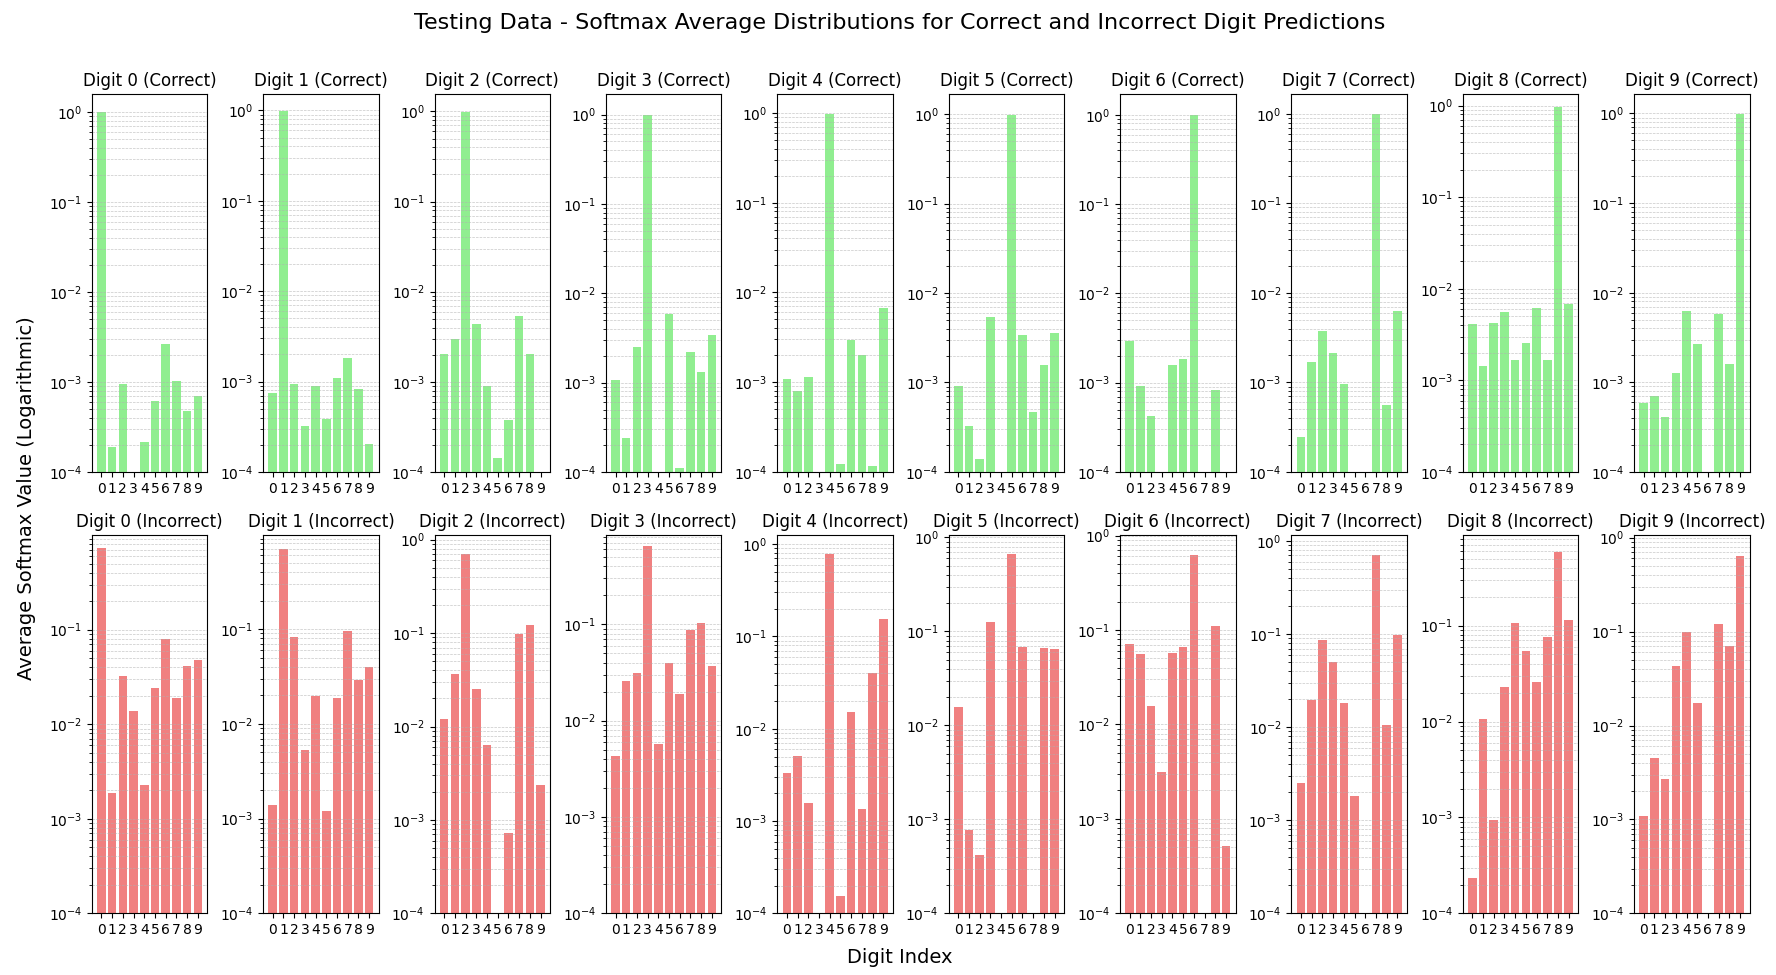
\includegraphics[width=0.99\columnwidth]{Figures/MNIST_Softmax_Averages_Testing.png}
%     \caption{Please zoom in for detail. Average Softmax Probabilities for Correctly and Incorrectly Classified Digits in the MNIST Testing Dataset.}
%     \label{fig:MNIST_Softmax_Averages_Testing}
% \end{figure}

%%%%%%%%%%%%%%%%%%%%%%%%%%%%%%%%%%%%%%%%%%%%%%%%%%%%%%%%%%%%%%%
% Average Softmax Probabilities for Correctly and Incorrectly %
% Classified Classes in the CIFAR10 dataset                   %
%%%%%%%%%%%%%%%%%%%%%%%%%%%%%%%%%%%%%%%%%%%%%%%%%%%%%%%%%%%%%%%

% Plot generated by function call
% single_plot_accuracy_decrements(accuracy_results, overall_results, labels=class_labels, dataset="CIFAR10", save=True)

% \begin{figure}[ht]
%     \centering    
%     \includegraphics[width=0.99\columnwidth]{Figures/CIFAR10_single_plot_accuracy_decrements.png}
%     \caption{Single plot Accuracy decrements}   \label{fig:CIFAR10_single_plot_accuracy_decrements}
% \end{figure}

% Function call to generate plot
% plot_centroid_distance_bars(train_correct_predictions, 
                            % train_incorrect_predictions, 
                            % labels=class_labels, 
                            % color1='lightblue', 
                            % color2='lightcoral', 
                            % data="CIFAR10 Training Data", 
                            % save=True, 
                            % filename='CIFAR10_training_plot_centroid_distance_bars.png')


% moved to methods for a better spread of images
% \begin{figure}[ht]
%     \centering
%     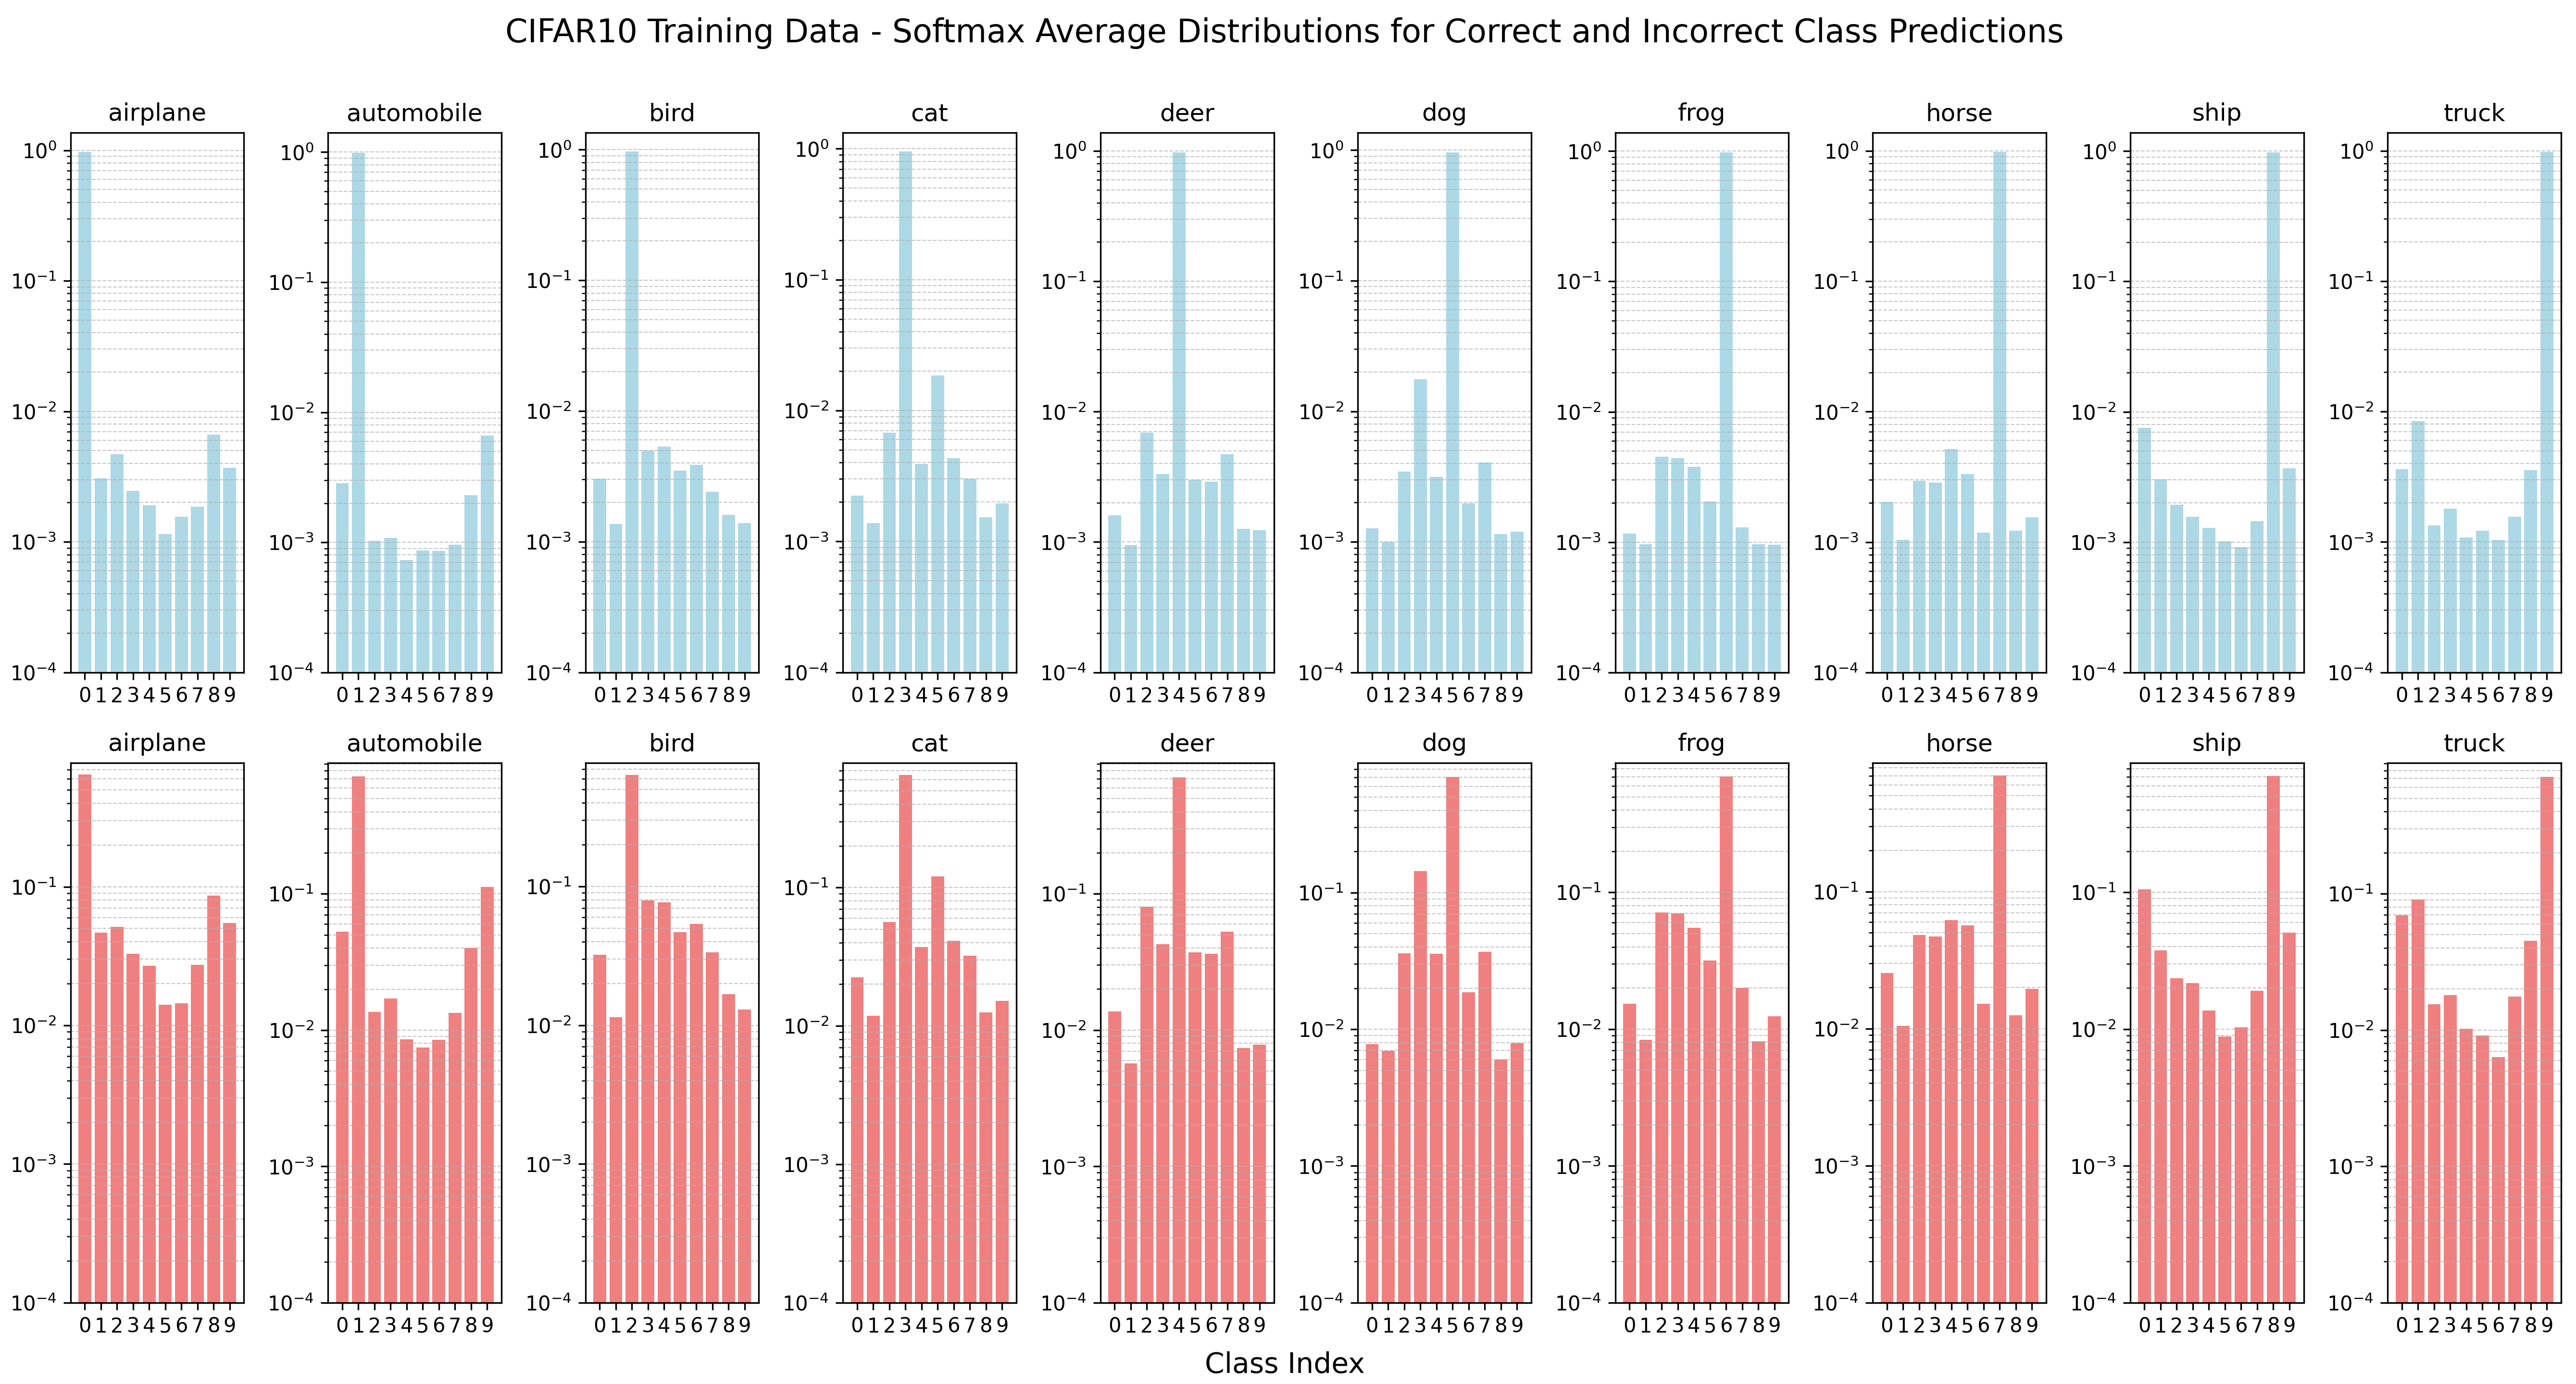
\includegraphics[width=0.95\columnwidth]{Figures/CIFAR10_training_plot_centroid_distance_bars.png}
%     \caption{Please zoom in for detail. Average Softmax Probabilities for Correctly and Incorrectly Classified Classes in the CIFAR-10 Training Dataset}
%     \label{fig:CIFAR10_training_plot_centroid_distance_bars.png}
% \end{figure}

% Function call to generate plot
% plot_centroid_distance_bars(test_correct_predictions, 
%                             test_incorrect_predictions, 
%                             labels=class_labels, 
%                             color1='lightgreen', 
%                             color2='lightcoral', 
%                             data="CIFAR10 Testing Data", 
%                             save=True, 
%                             filename='CIFAR10_testing_plot_centroid_distance_bars.png')

% Moved to Supplementary Material
% \begin{figure}[ht]
%     \centering
%     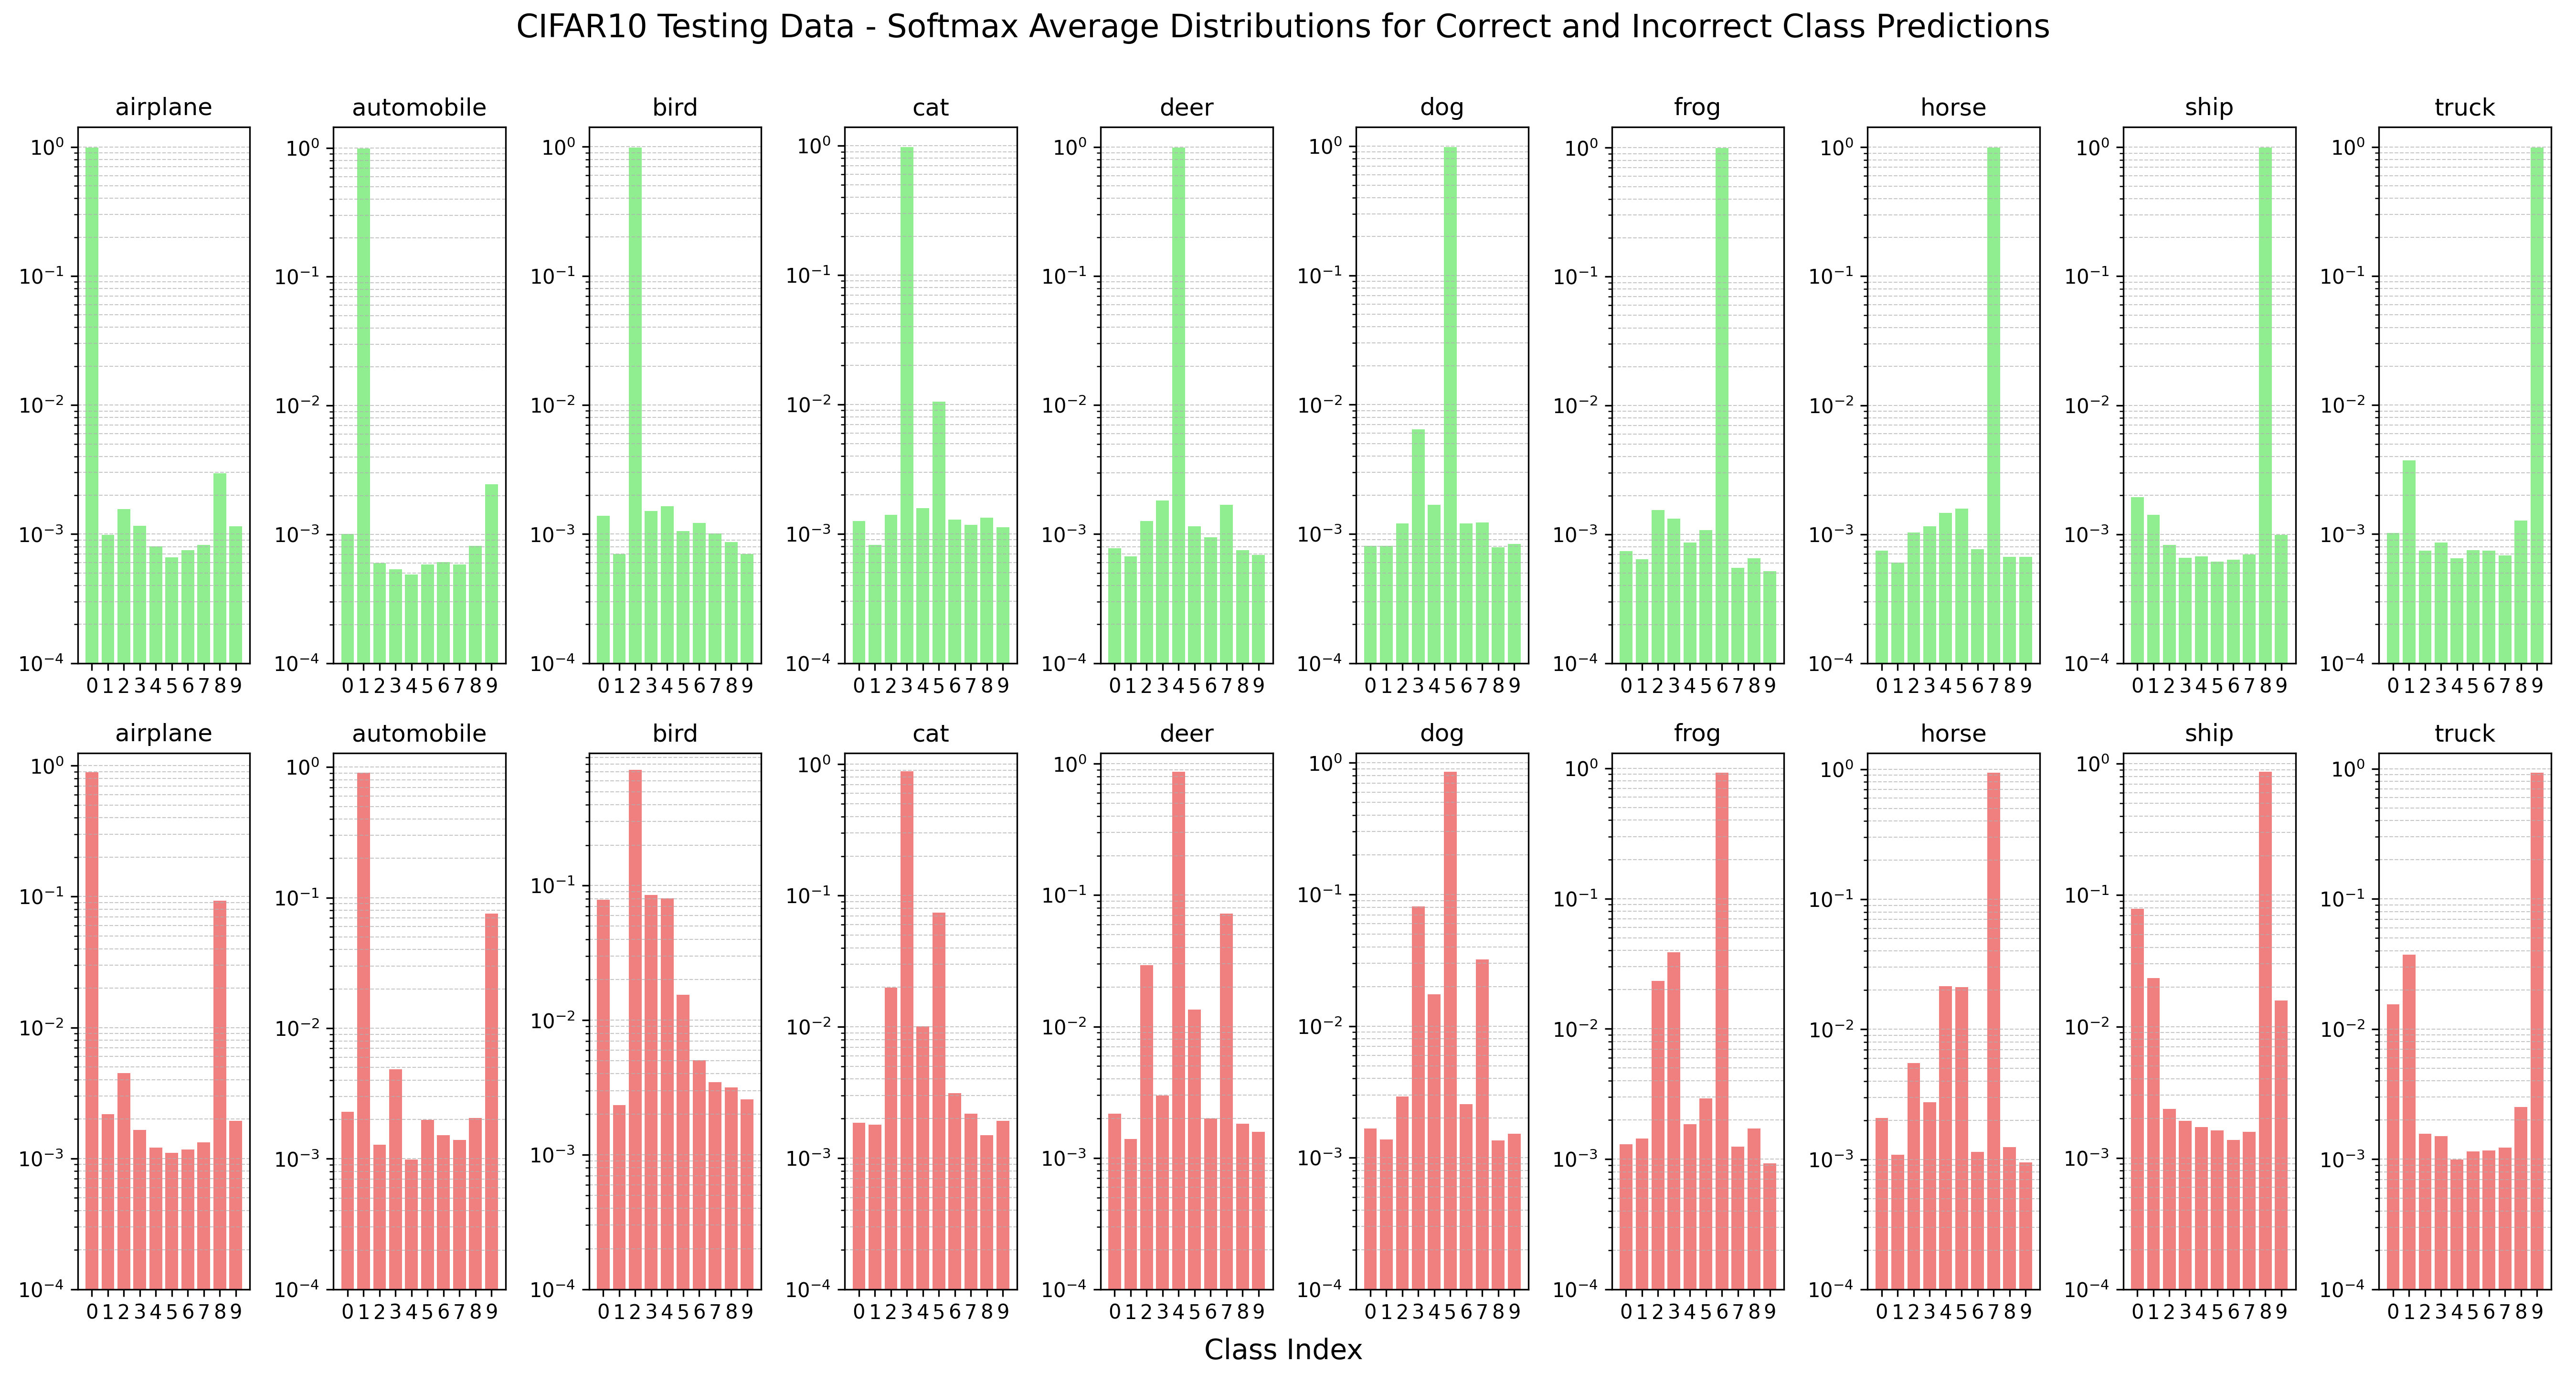
\includegraphics[width=0.95\columnwidth]{Figures/CIFAR10_testing_plot_centroid_distance_bars.png}
%     \caption{Please zoom in for detail. Average Softmax Probabilities for Correctly and Incorrectly Classified classes in the CIFAR-10 Testing Dataset}
%     \label{fig:CIFAR10_testing_plot_centroid_distance_bars.png}
% \end{figure}

% is a bar chart representing the mean softmax distances to class centroid for all correct (green) and all incorrect (red) classifications from the ViT model trained on CIFAR-10 data. 

% The softmax distribution bar charts provide a view of the model's confidence and uncertainty in its predictions. The distinct patterns observed for correct and incorrect classifications offer valuable information about the model's decision-making process.

For the CIFAR-10 we observe similar results. For correctly classified instances, the average softmax value corresponding to the true digit class is significantly higher compared to the softmax values of the other digit classes. This observation holds true across all digit classes in both the testing and training datasets. The pronounced difference in magnitudes indicates that the model assigns a high level of confidence to the correct predictions, with the predicted probability for the true class being orders of magnitude larger than the probabilities assigned to the other classes.

In contrast, for incorrectly classified instances, the average softmax values exhibit a more even distribution across the digit classes. While the softmax value for the predicted class is still relatively high, the softmax values for the other classes are notably closer in magnitude, as evident from the shorter bars on the logarithmic scale. This suggests that when the model makes an incorrect prediction, it assigns more substantial probabilities to multiple classes, indicating a higher level of uncertainty or confusion in the decision-making process.
Figures \ref{fig:CIFAR10_training_plot_centroid_distance_bars.png} and \ref{fig:CIFAR10_testing_plot_centroid_distance_bars.png} bar charts show the average softmax distributions for correct (green/blue) and incorrect (red) class predictions in both the testing and training CIFAR-10 datasets.

Comparing the testing and training datasets, we observe similar patterns in the softmax distance distributions for both correct and incorrect predictions. The consistency of these patterns suggests that our approach is consistent across datasets and models. 

The analysis of softmax distance distributions may be taken as an insight into the model's decision-making process. The difference in the softmax values between correct and incorrect predictions highlights the model's ability to discriminate between classes when it makes accurate predictions. On the other hand, the more evenly distributed softmax values for incorrect predictions suggest that the model struggles to make clear distinctions between classes in those cases, assigning considerable probabilities to multiple digits, where our proposed thresholding method may be an additional tool to help evaluate predictions in different settings.

%%%%%%%%%%%%%%%%%%%%%%%%%%%%%%
% CONCLUSION AND FUTURE WORK %
%%%%%%%%%%%%%%%%%%%%%%%%%%%%%%

\section{Conclusions and Future Work}

We presented a simple approach to thresholding accuracy in an image classification setting, by training two distinct network architectures, on two distinct datasets, and showing our results are consistent across both scenarios.
We demonstrated the steps required to effectively create class clusters by initialising centroids with the mean of correct class predictions for each distinct class, where the K-Means algorithm quickly converges with good cluster separation.
A threshold was proposed to ensure predictions below threshold are safe, at a small cost of labelling as incorrect a small number of correct predictions at or above threshold.

We posit that the optimal threshold is domain-dependent and should be determined by domain experts who are equipped to balance the efficiency of automated decision-making against the necessity for time-intensive human judgment, taking into account the specific stakes involved.

We are applying the concepts discussed in this study to autonomous system safety, in the context of self-driving cars using the CARLA simulator, and constituent tasks in the decision-making stack, such as image classification and segmentation, where our methodology aims to enhance system safety by identifying scenarios, including OOD scenarios, where human judgment is preferable to the autonomous system’s assessment.

%our approach may help make such systems safer, by deferring to human judgement what may not be safely assessed by the autonomous system.

% Finally, we are considering the softmax output as a training dataset in itself, for a simple multi-layer perceptron binary classifier, to compare and contrast the softmax distance approach, and a regressor network combined with our current approach, to provide a quantity e.g. sigmoid function output as a weight to further study optimal threshold values.

We plan to integrate centroid distance, entropy, and Entropy Apex - a point equidistant to all centroids - proximity metrics, where a maximal entropy region is expected to be identified, the combined metrics providing a weighted confidence. Finally, we plan to introduce noise, and expect predictions will move from areas of low entropy nearer to centroids, to areas of higher entropy, nearer to the apex. 

\bibliography{aaai25}

\appendix
%%%%%%%%%%%%
% APPENDIX %
%%%%%%%%%%%%

\clearpage
\section{Supplementary Materials - Submission Number: 14590}

\subsection{Extended results}

Addional results that complement previously shown results, are displayed in this section.

\begin{figure}[ht]
    \centering
    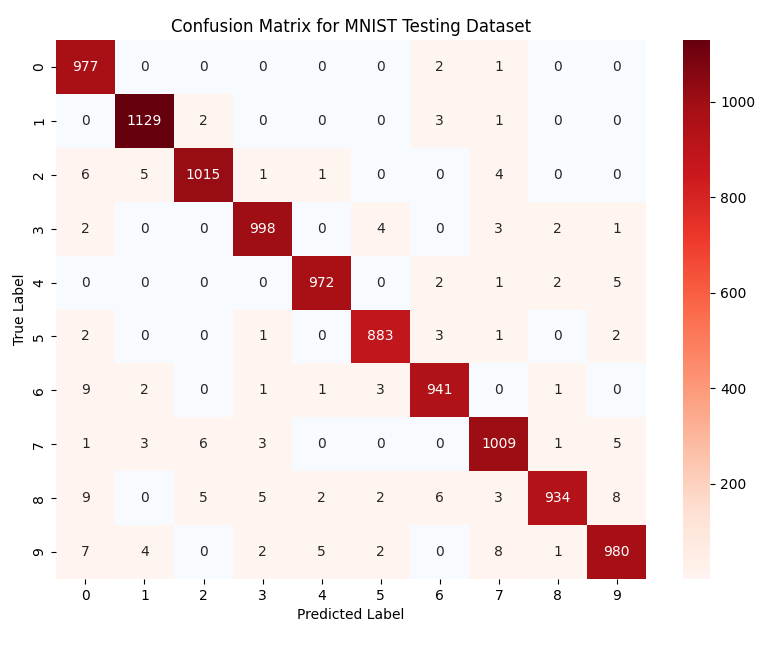
\includegraphics[width=0.99\columnwidth]{Figures/mnist_testing_confusion_matrix.png}
    \caption{Confusion matrices for the MNIST classification model on the training dataset. The matrices display the true labels on the vertical axis and the predicted labels on the horizontal axis. The diagonal elements represent correctly classified instances, while the off-diagonal elements indicate misclassifications. The corresponding confusion matrix for the testing dataset is provided in the supplementary materials.}
    \label{fig:mnist_testing_confusion_matrix}
\end{figure}

The confusion matrix for the CIFAR-10 testing dataset in Figure \ref{fig:cifar10_testing_confusion_matrix}. Examining the testing dataset, the model achieves good classification success, with perfect recognition of 'frog' class. Misclassifications are present but considerably reduced compared to the training dataset, particularly for pairs such as 'truck' and 'automobile', as well as 'cat' and 'dog'. The reduced confusion in the test set is also reflected in the softmax distance to cluster centroid.

\begin{figure}[ht]
    \centering   
    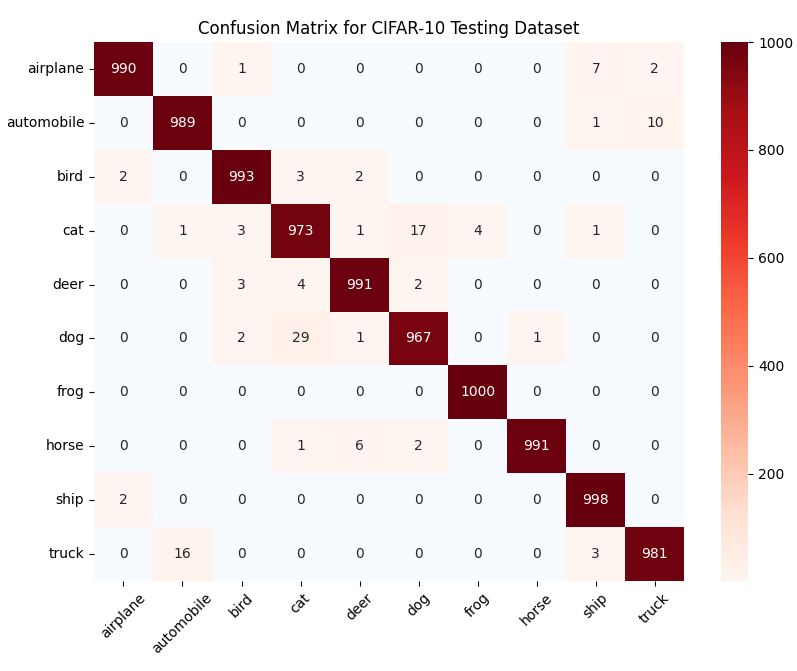
\includegraphics[width=0.99\columnwidth]{Figures/cifar10_testing_confusion_matrix.png}
    \caption{Confusion matrix for the CIFAR-10 classifier model training dataset dataset dataset correct and incorrect classifications. The corresponding matrix for the testing dataset is given in the supplementary materials.}
    \label{fig:cifar10_testing_confusion_matrix}
\end{figure}

%%%%%%%%%%%%%%%%%%%%%%%%%%%%%%%%%%%%%%%%%%%
% COMBINED CIFAR10 MNIST ACCURACY VS MEAN %
% CLASS PREDICTION DISTANCE TO CENTROID   %
%%%%%%%%%%%%%%%%%%%%%%%%%%%%%%%%%%%%%%%%%%%

Figures \ref{fig:CIFAR10_plot_accuracy_vs_distance_linear_fit} and \ref{fig:mnist_plot_accuracy_vs_distance_linear_fit} suggest how both the trained CNN and ViT models achieves higher predictive accuracy for classes that have lower softmax distance to their respective class centroids, compared to classes for which the models obtain lower predictive accuracy.

% In the context of the MNIST dataset, the derived linear functions from the training and testing data exhibit a negative correlation between the classification accuracy and the mean class distances to the centroids. Specifically, the training data is described by the function $ y = -0.806x + 1.009 $, and the testing data by $ y = -0.677x + 1.004 $. The negative coefficients of the linear terms $ -0.806 $ and $ -0.677 $, respectively) indicate that an increase in the mean distance to the centroid correlates with a decrease in classification accuracy for both datasets.

The scatter plots show the relationship between classification accuracy and mean class distance to the centroid for the CIFAR-10 MNIST dataset. Training data (blue dots) and testing data (green dots) are each fitted with a linear regression line, demonstrating a negative correlation where increased mean distance corresponds to decreased accuracy. For the CNN/MNIST experiment, the steeper slope of the training data fit (-0.806) compared to the testing data fit (-0.677) reflects the greater accuracy and more compact cluster obtained from the correct test predictions compared to the cluster obtained from correct training predictions, noting that both training and testing data use centroids obtained from the correctly classified examples in the training dataset.

These results show an inverse relationship: as the mean distance from the data points in a class to their centroid increases, the propensity for correct classification diminishes. This could be due to the spread of data points within a class – greater distances from the centroid reflect a larger variance within the class, potentially making it more challenging for the classifier to identify the defining characteristics of each class accurately.

The CIFAR-10 linear fit is steeper as can be observed by the y axis values, although it can be argued provides a better fit.

% Plot created manually from MNIST and CIFAR10 plots created by function plot_accuracy_vs_distance_linear_fit
\begin{figure*}[ht]
    \centering
    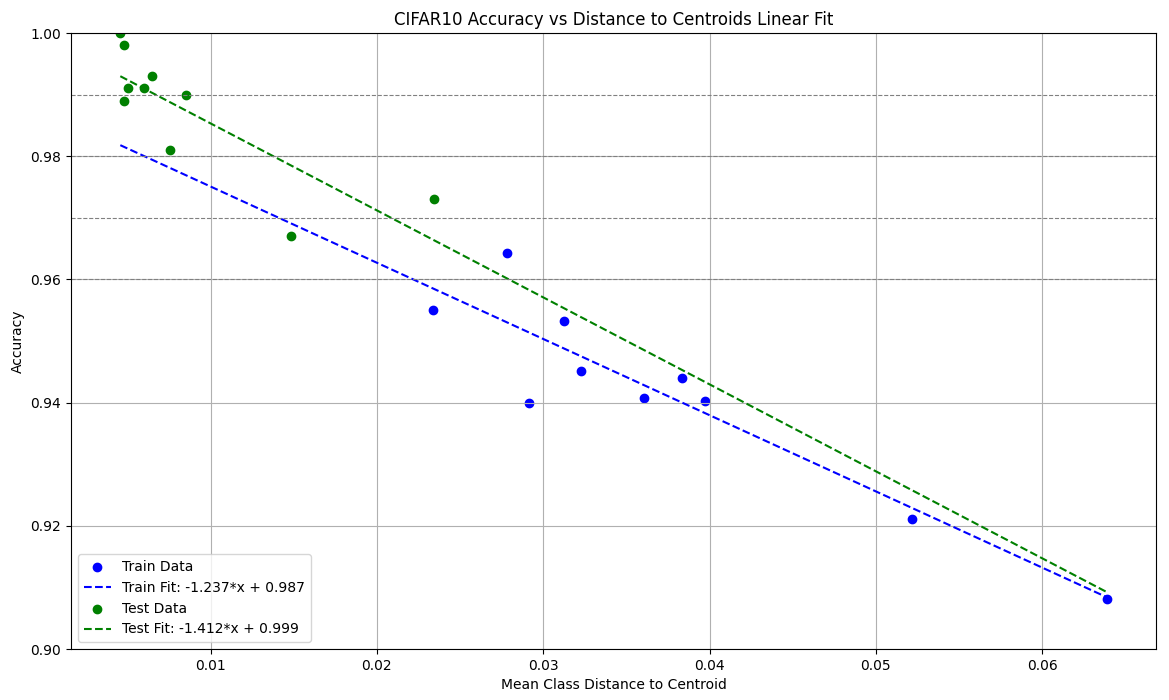
\includegraphics[width=0.99\textwidth]{Figures/CIFAR10_plot_accuracy_vs_distance_linear_fit.png}
    \caption{Expected accuracy linear fit based on prediction softmax distance to class centroid. ViT/CIFAR-10 training dataset predictions}
\label{fig:CIFAR10_plot_accuracy_vs_distance_linear_fit}
\end{figure*}

\begin{figure*}[ht]
    \centering
    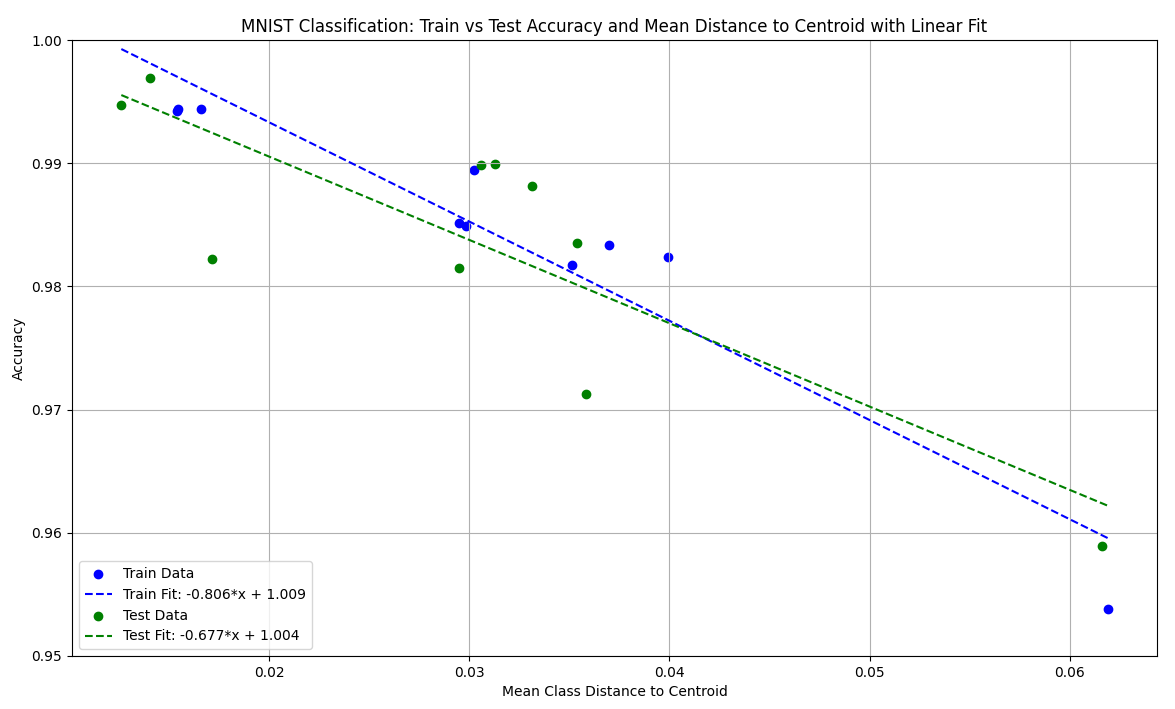
\includegraphics[width=0.99\textwidth]{Figures/mnist_plot_accuracy_vs_distance_linear_fit.png}
    \caption{Expected accuracy linear fit based on prediction softmax distance to class centroid. CNN/MNIST training dataset predictions.}
\label{fig:mnist_plot_accuracy_vs_distance_linear_fit}
\end{figure*}

%Combined_CIFAR10_MNIST_Classification_Train_Test_Accuracy_Mean_Distance_to_Centroid_Linear_Fit.png

% \subsection{Overlap table CIFAR discussion 2}

% %%%%%%%%%%%%%%%
% % LATEX TABLE %
% %%%%%%%%%%%%%%%

% % Table generated by function call
% % centroid_distance_overlap_latex(d2c_train_correct, 
% %                                 d2c_train_incorrect, 
% %                                 d2c_test_correct, 
% %                                 d2c_test_incorrect, 
% %                                 labels=class_labels,
% %                                 caption='CIFAR10 centroid distances overlap count for correct predictions above incorrect threshold'
% %                             ) 

% \begin{table}[htbp]
% \centering
% \begin{tabular}{|c|c|c|c|c|c|c|}
% \hline
% Class & \multicolumn{3}{c|}{Train Data - Train Centroids} & \multicolumn{3}{c|}{Test Data - Train Centroids} \\
% \hline
%  & Count & Total & Overlap & Count & Total & Overlap \\
% \hline
% plane & 13 & 4252 & 0.31\% & 1 & 990 & 0.10\% \\
% auto & 1 & 4326 & 0.02\% & 0 & 989 & 0.00\% \\
% bird & 9 & 4216 & 0.21\% & 0 & 993 & 0.00\% \\
% cat & 20 & 4103 & 0.49\% & 2 & 973 & 0.21\% \\
% deer & 14 & 4255 & 0.33\% & 0 & 991 & 0.00\% \\
% dog & 11 & 4157 & 0.26\% & 1 & 967 & 0.10\% \\
% frog & 11 & 4310 & 0.26\% & 0 & 1000 & 0.00\% \\
% horse & 12 & 4223 & 0.28\% & 0 & 991 & 0.00\% \\
% ship & 11 & 4258 & 0.26\% & 0 & 998 & 0.00\% \\
% truck & 10 & 4251 & 0.24\% & 0 & 981 & 0.00\% \\
% \hline
% Totals & 112 & 42351 & 0.26\% & 4 & 9873 & 0.04\% \\
% \hline
% \end{tabular}
% \caption{CIFAR10 centroid distances overlap count for correct predictions above incorrect threshold}
% \label{tab:centroid_distance_overlap}
% \end{table}

\begin{table*}[htbp]
\centering
\begin{tabular}{|c|c|c|c|c|c|c|}
\hline
Digit & \multicolumn{3}{c|}{Train Data - Train Centroids} & \multicolumn{3}{c|}{Test Data - Train Centroids} \\
\hline
 & Count & Total & Overlap & Count & Total & Overlap \\
\hline
0 & 2 & 5890 & 0.03\% & 1 & 977 & 0.10\% \\
1 & 0 & 6704 & 0.00\% & 0 & 1129 & 0.00\% \\
2 & 1 & 5859 & 0.02\% & 0 & 1015 & 0.00\% \\
3 & 3 & 6019 & 0.05\% & 1 & 998 & 0.10\% \\
4 & 0 & 5755 & 0.00\% & 0 & 972 & 0.00\% \\
5 & 5 & 5339 & 0.09\% & 0 & 883 & 0.00\% \\
6 & 2 & 5884 & 0.03\% & 1 & 941 & 0.11\% \\
7 & 2 & 6199 & 0.03\% & 0 & 1009 & 0.00\% \\
8 & 12 & 5581 & 0.22\% & 1 & 934 & 0.11\% \\
9 & 1 & 5844 & 0.02\% & 0 & 980 & 0.00\% \\
\hline
Totals & 28 & 59074 & 0.05\% & 4 & 9838 & 0.04\% \\
\hline
\end{tabular}
\caption{MNIST counts of correctly classified training and testing image predictions and counts with distance to centroids equal or above error threshold.}
\label{tab:centroid_distance_overlap_mnist}
\end{table*}

\begin{table*}[htbp]
\centering
\begin{tabular}{|c|c|c|c|c|c|c|}
\hline
Class & \multicolumn{3}{c|}{Train Data - Train Centroids} & \multicolumn{3}{c|}{Test Data - Train Centroids} \\
\hline
 & Count & Total & Overlap & Count & Total & Overlap \\
\hline
plane & 13 & 4252 & 0.31\% & 1 & 990 & 0.10\% \\
auto & 1 & 4326 & 0.02\% & 0 & 989 & 0.00\% \\
bird & 9 & 4216 & 0.21\% & 0 & 993 & 0.00\% \\
cat & 20 & 4103 & 0.49\% & 2 & 973 & 0.21\% \\
deer & 14 & 4255 & 0.33\% & 0 & 991 & 0.00\% \\
dog & 11 & 4157 & 0.26\% & 1 & 967 & 0.10\% \\
frog & 11 & 4310 & 0.26\% & 0 & 1000 & 0.00\% \\
horse & 12 & 4223 & 0.28\% & 0 & 991 & 0.00\% \\
ship & 11 & 4258 & 0.26\% & 0 & 998 & 0.00\% \\
truck & 10 & 4251 & 0.24\% & 0 & 981 & 0.00\% \\
\hline
Totals & 112 & 42351 & 0.26\% & 4 & 9873 & 0.04\% \\
\hline
\end{tabular}
\caption{CIFAR10 counts of correctly classified training and testing image predictions and counts with distance to centroids equal or above error threshold.}
\label{tab:centroid_distance_overlap}
\end{table*}

Table \ref{tab:centroid_distance_overlap_mnist} presents an analysis of the counts and percentages of correctly classified images in the training and testing datasets that have softmax distances to their respective class centroids above a certain threshold. The threshold is determined by the nearest softmax distance to the centroid for the incorrectly classified classes.

The table is divided into two main sections: "Train Data - Train Centroids" and "Test Data - Train Centroids." For each section, the table provides the count of images that satisfy the threshold condition, the total number of images in each class, and the percentage of overlap (i.e., the proportion of images above the threshold relative to the total count).

Looking at the "Train Data - Train Centroids" section, we observe that the overlap percentages are relatively low, ranging from 0.00\% to 0.22\%. This suggests that only a small fraction of the correctly classified training images have softmax distances to their centroids above the threshold set by the incorrectly classified images. The highest overlap is observed for digit class 8, with 12 out of 5,581 images (0.22\%) having distances above the threshold.

Similarly, in the "Test Data - Train Centroids" section, the overlap percentages are even lower, ranging from 0.00\% to 0.11\%. This indicates that the trained model is able to correctly classify the majority of the test images while maintaining a distance to the centroids below the threshold set by the incorrectly classified images. The highest overlap in the test data is observed for digit classes 6 and 8, with 1 out of 941 (0.11\%) and 1 out of 934 (0.11\%) images, respectively, having distances above the threshold.

The Totals summarise the overall counts and overlap percentages across all digit classes. For the training data, 28 out of 59,074 images (0.05\%) have distances above the threshold, while for the test data, only 4 out of 9,838 images (0.04\%) exceed the threshold.

The low overlap percentages indicate that the majority of the correctly classified images are well-separated from the incorrectly classified images in terms of their softmax distances to the centroids. This analysis provides insights into the softmax distance being a proxy to distinguish between between correct and incorrect digit classifications based on the proximity of the images to their respective class centroids in the softmax distance space. The same analysis applies to Table \ref{tab:centroid_distance_overlap}. Most indicative of the consistency of the suggested approach is than both CIFAR-10 and MNIST present an overlap of 0.04\% for correctly classified images at or above threshold. Note we tag the images in the overlap as incorrectly classified, for the sake of assuring that all softmax distances to cluster centroid below threshold are correct classifications.

\begin{figure*}[ht]
    \centering
    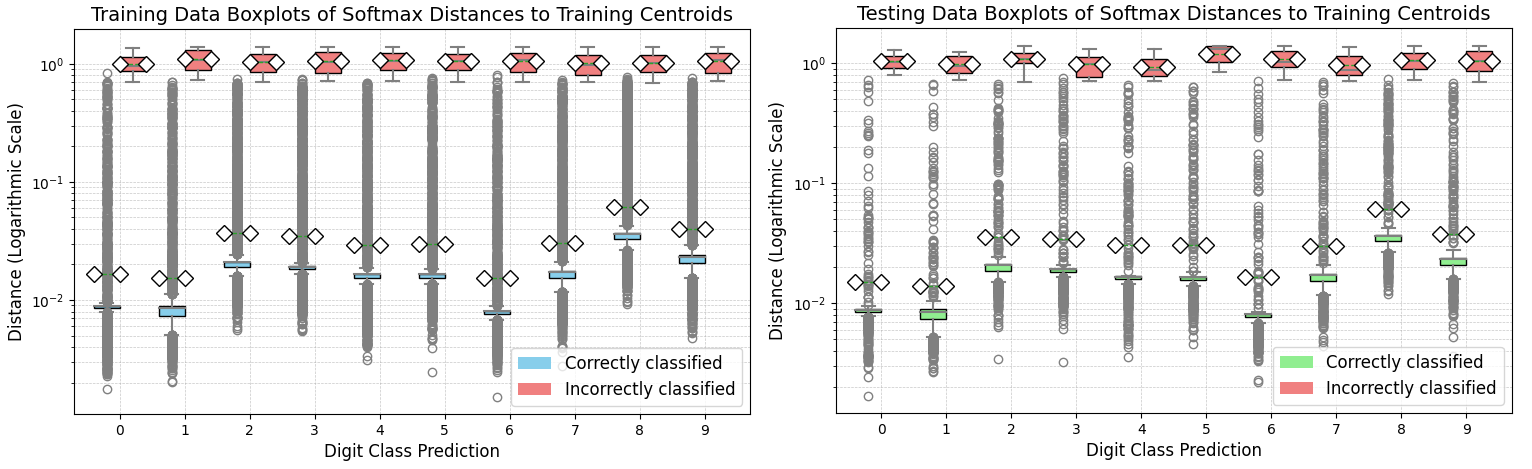
\includegraphics[width=0.99\textwidth]{Figures/MNIST_boxplots_side_by_side_x2.png}   \captionsetup{justification=raggedright,singlelinecheck=false}
    \caption{Distribution of Distances to Centroids for Correctly and Incorrectly Classified Instances in Training and Testing MNIST data, where training data is on the left and testing data is displayed on the right. Distances on y axis are shown on a logarithmic scale. Centroids are obtained from correctly classified training examples, then used for both training and testing datasets, a cluster is not created from the testing softmax distances. }
    \label{fig:MNIST_boxplots_side_by_side_x2}
\end{figure*}

% AVERAGE SOFTMAX OUTPUTS CNN/MNIST, ViT/CIFAR-10, training and testing datasets

% function call
% plot_digit_averages(test_correct_predictions, test_incorrect_predictions, color1='lightgreen', color2='lightcoral', data="Testing Data")
\begin{figure*}[ht]
    \centering
    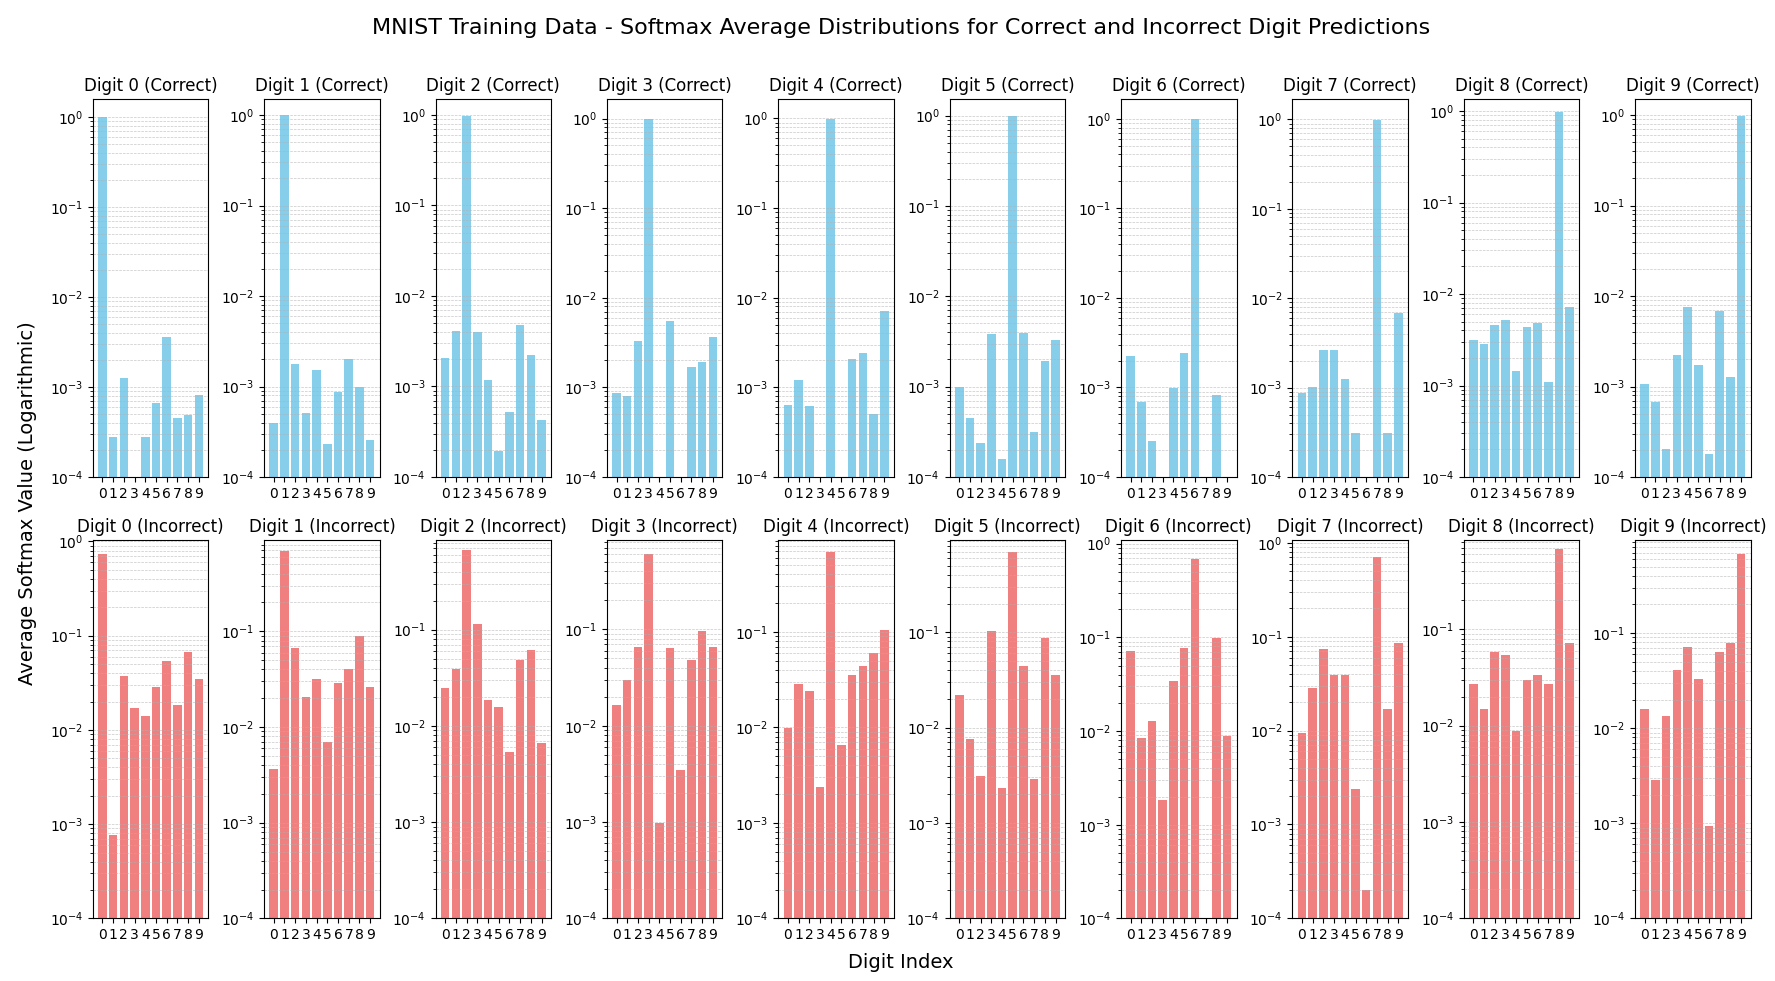
\includegraphics[width=0.99\textwidth]{Figures/MNIST_Softmax_Averages_Training.png}
    \caption{Average Softmax Probabilities for Correctly and Incorrectly Classified Digits in the MNIST Testing Dataset.}
    \label{fig:MNIST_Softmax_Averages_Training}
\end{figure*}

Figure \ref{fig:MNIST_Softmax_Averages_Training} shows the average softmax probabilities for each digit class (0 to 9) in the MNIST training dataset, separated into correctly classified instances (top row) and incorrectly classified instances (bottom row). The probabilities are displayed on a logarithmic scale. For correctly classified digits, the highest average probability is observed for the corresponding true digit class, indicating strong confidence in the correct predictions. In contrast, for incorrectly classified digits, the average probabilities are more evenly distributed across different digit classes, suggesting lower confidence and potential confusion between similar-looking digits.
Figure \ref{fig:MNIST_Softmax_Averages_Testing} is the corresponding plot for the MNIST testing dataset.

% function call
% plot_digit_averages(test_correct_predictions, test_incorrect_predictions, color1='lightgreen', color2='lightcoral', data="Testing Data")
\begin{figure}[ht]
    \centering
    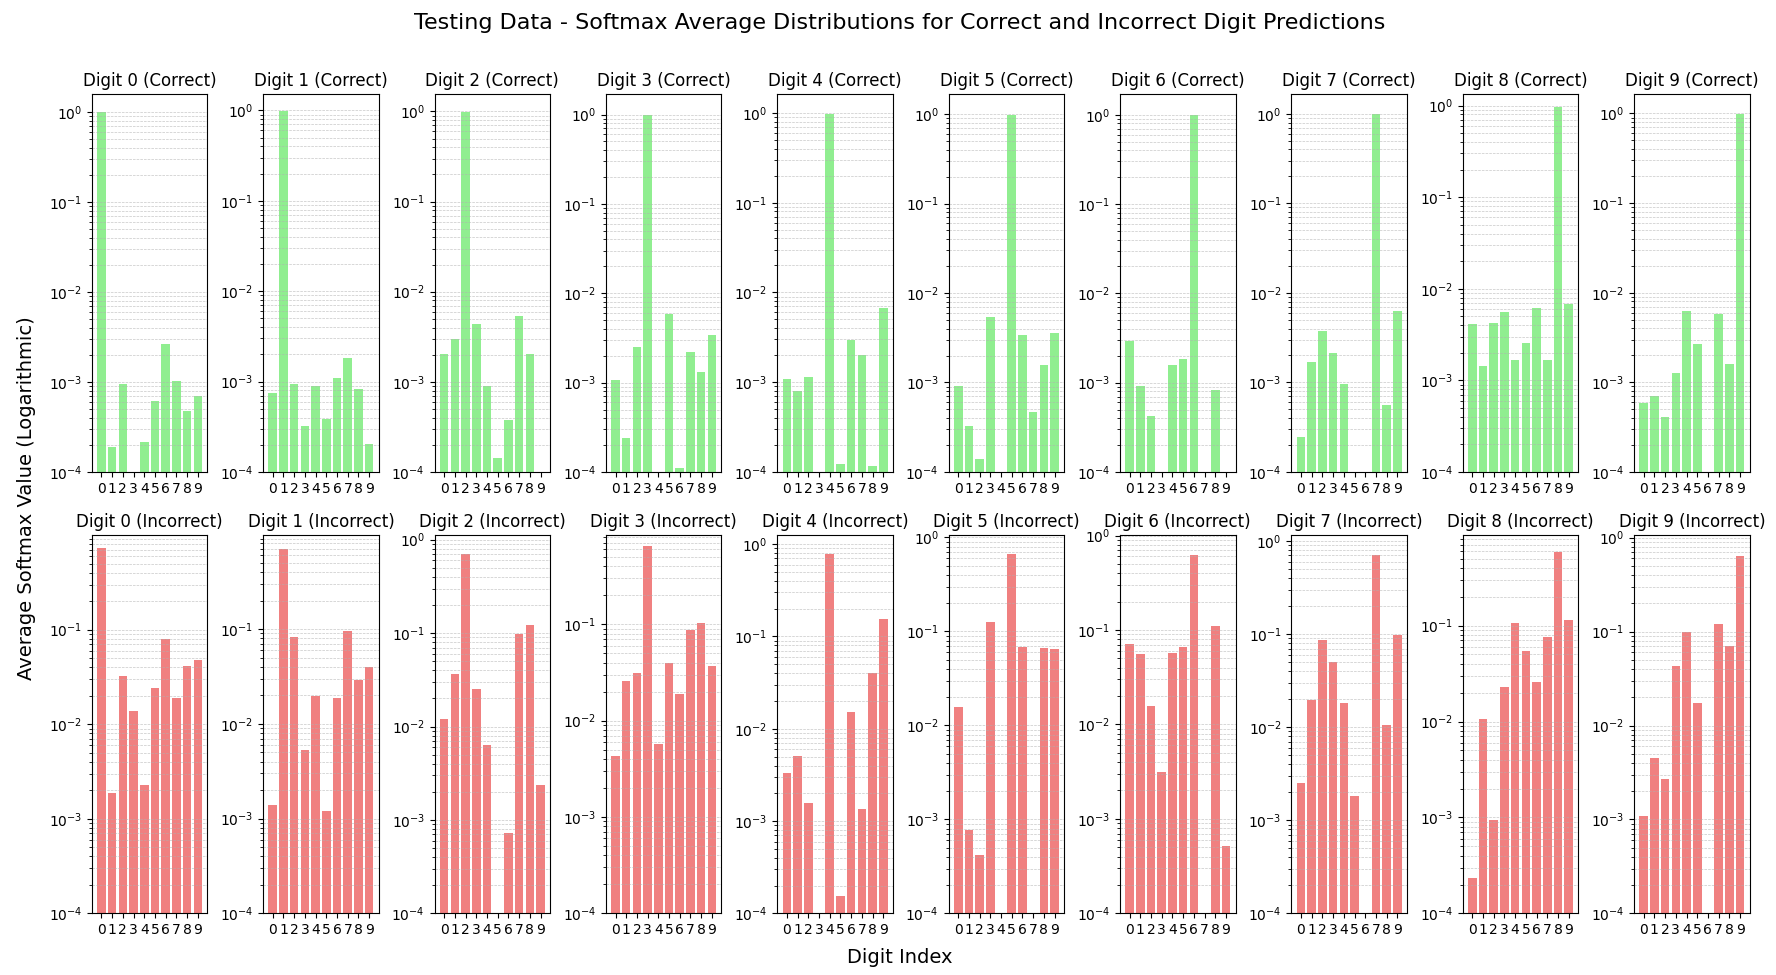
\includegraphics[width=0.99\textwidth]{Figures/MNIST_Softmax_Averages_Testing.png}
    \caption{Average Softmax Probabilities for Correctly and Incorrectly Classified Digits in the MNIST Testing Dataset.}
    \label{fig:MNIST_Softmax_Averages_Testing}
\end{figure}


\begin{figure}[ht]
    \centering
    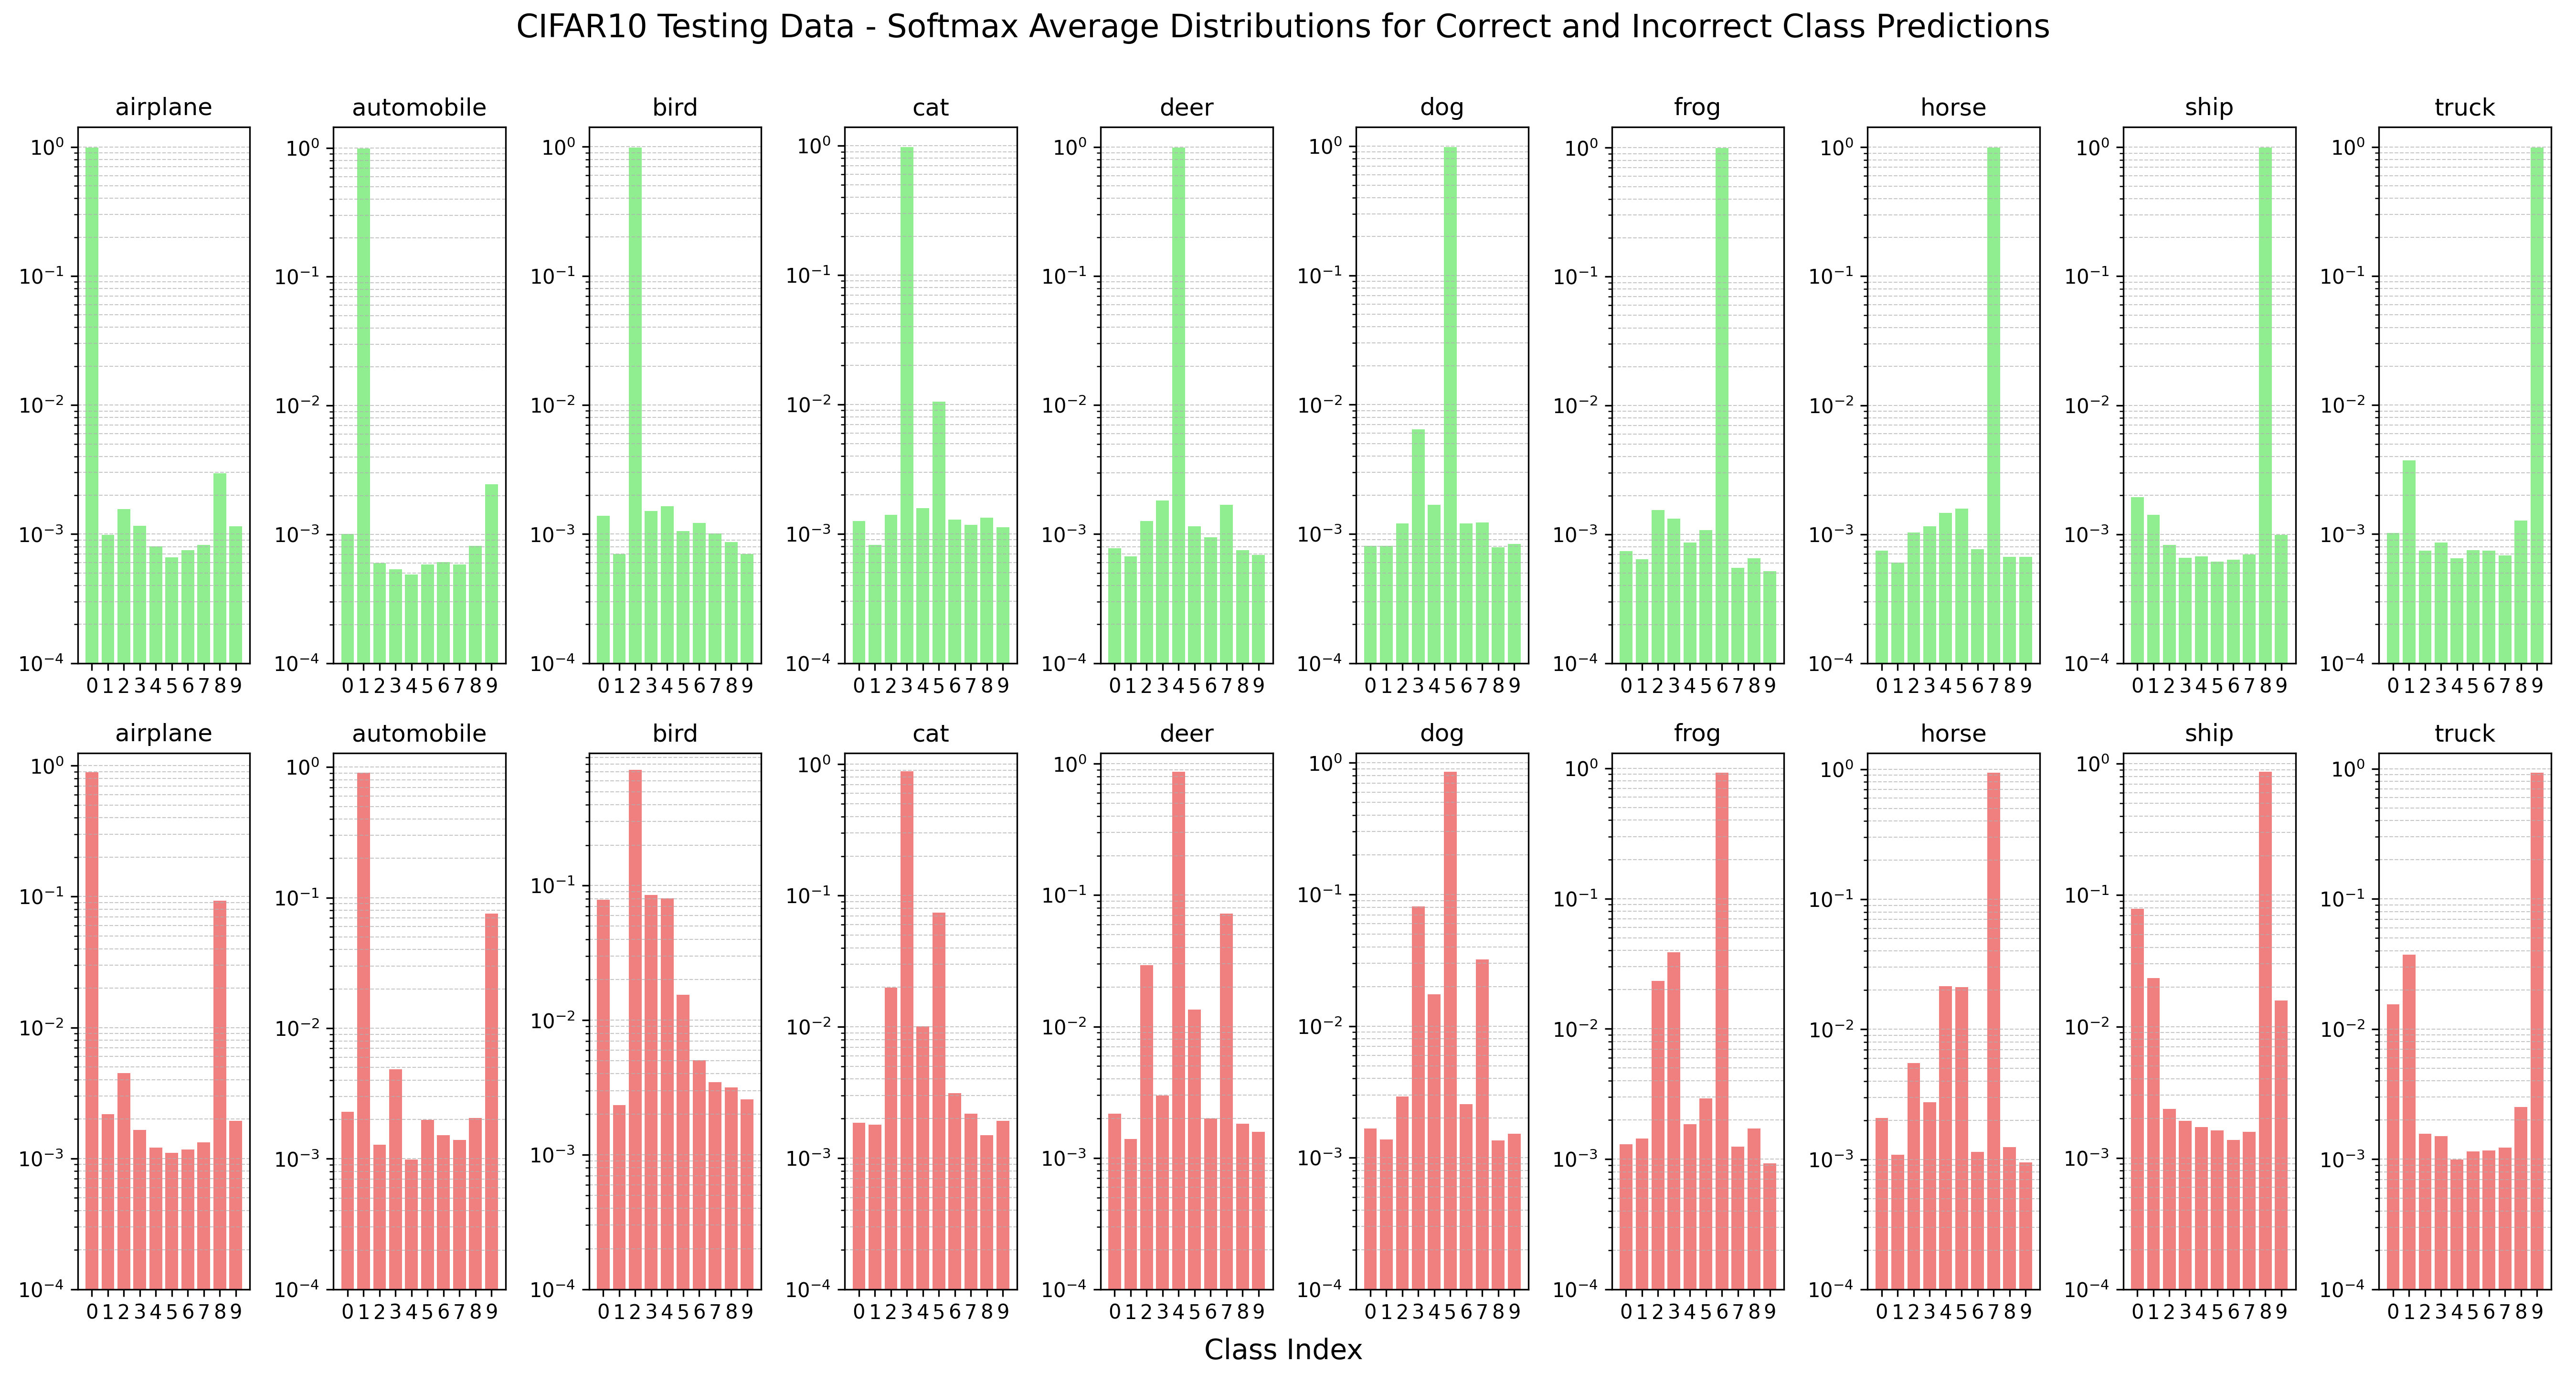
\includegraphics[width=0.99\textwidth]{Figures/CIFAR10_testing_plot_centroid_distance_bars.png}
    \caption{Please zoom in for detail. Average Softmax Probabilities for Correctly and Incorrectly Classified classes in the CIFAR-10 Testing Dataset}
    \label{fig:CIFAR10_testing_plot_centroid_distance_bars.png}
\end{figure}

%%%%%%%%%%%%%%%%%%%%%%%%%%%%%%%%%%%%%%%%%%%
% COMBINED CIFAR10 MNIST ACCURACY VS MEAN %
% CLASS PREDICTION DISTANCE TO THRESHOLD  %
%%%%%%%%%%%%%%%%%%%%%%%%%%%%%%%%%%%%%%%%%%%

% Plot created by joining plots created by plot_accuracy_vs_distance_linear_fit

\begin{figure*}[ht]
    \centering
    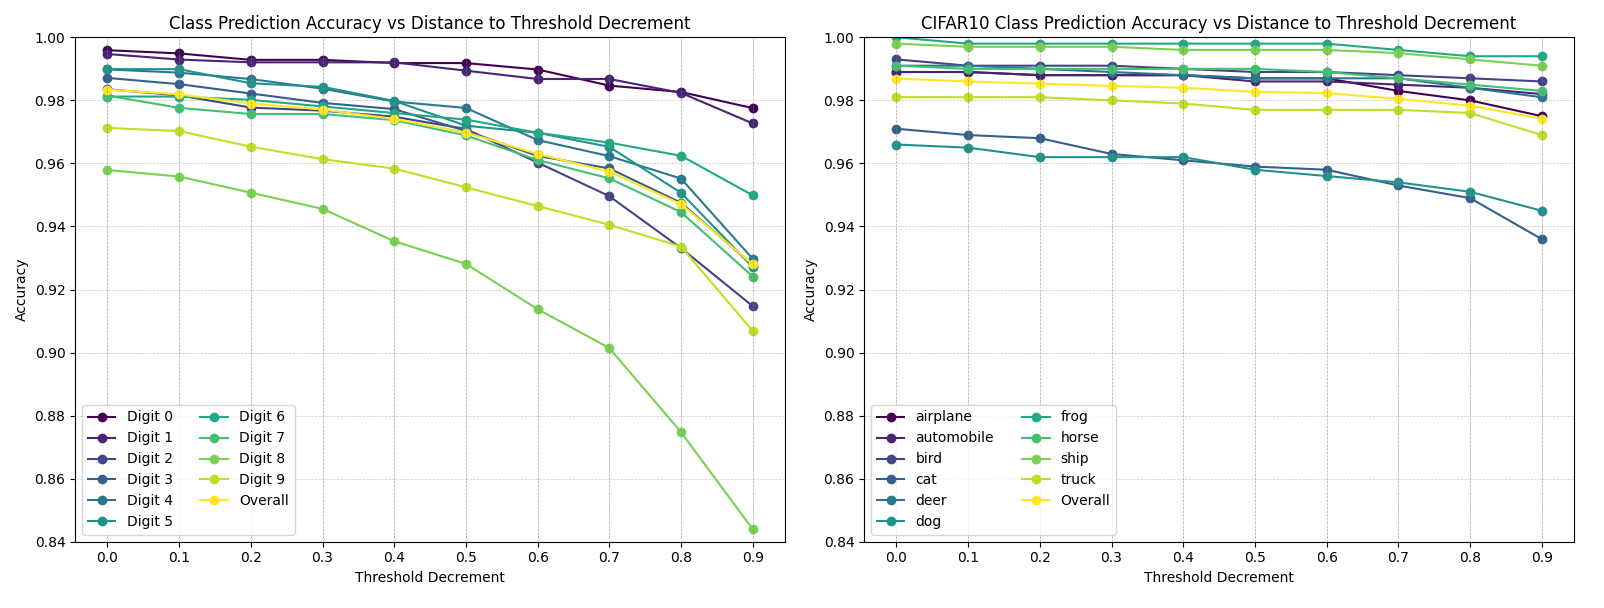
\includegraphics[width=0.99\textwidth]{Figures/Combined_CIFAR10_MNIST_single_plot_accuracy_decrements.png}
    \caption{Expected accuracy decrease as a result of threshold decrease. MNIST data is on the left, CIFAR-10 is on the right. The x axis shows the threshold decrement in factors of 0.1, that is, at 0.1 the threshold is 90\% of the original threshold while at 0.9 the threshold is 10\% of the original threshold and consequently neared to the class centroid.}
\label{fig:Combined_CIFAR10_MNIST_single_plot_accuracy_decrements.png}
\end{figure*}



\end{document}
